\documentclass{thesisclass}
\usepackage{adjustbox}  
\usepackage{tikz}
\usepackage{subcaption}
\usepackage{microtype}
\usepackage{amsmath}
%\usepackage{subfig}

% suppress subsubsection for contents
\setcounter{tocdepth}{2}
% suppress numbering for subsubsection{}
\setcounter{secnumdepth}{2}

% Based on thesisclass.cls of Timo Rohrberg, 2009
% ----------------------------------------------------------------
% Thesis - Main document
% ----------------------------------------------------------------


%% -------------------------------
%% |  Information for PDF file   |
%% -------------------------------
\hypersetup{
 pdfauthor={},
 pdftitle={},
 pdfsubject={Not set},
 pdfkeywords={Not set}
}

\newcommand{\tm}{\textsuperscript{\scriptsize\texttrademark}}
\newcommand{\reg}{\textsuperscript{\scriptsize\textregistered}}
%\newcommand{\copy}{\textsuperscript{\scriptsize\textcopyright}}

%% ---------------------------------
%% | Information about the thesis  |
%% ---------------------------------

\newcommand{\myname}{Amelie Wagner}
\newcommand{\mytitle}{Image-based segmentation\\ and localization\\ of surgical instruments\\ using deep neural networks
}

\newcommand{\reviewerone}{Prof. Dr.-Ing. Stefanie Speidel}
\newcommand{\reviewertwo}{Dr.-Ing. Sebastian Bodenstedt}
\newcommand{\advisor}{Isabel Funke}
% If there is a second advisor, uncomment in titlepage.tex!
\newcommand{\advisortwo}{?}

\newcommand{\timestart}{July 02, 2018}
\newcommand{\timeend}{November 03, 2018}
\newcommand{\submissiontime}{01. November 2018}


%% ---------------------------------
%% | ToDo Marker - only for draft! |
%% ---------------------------------
% Remove this section for final version!
%\setlength{\marginparwidth}{20mm}


%% --------------------------------
%% | Settings for word separation |
%% --------------------------------
% Help for separation:
% In  package the following hints are additionally available:
% "- = Additional separation
% "| = Suppress ligation and possible separation (e.g. Schaf"|fell)
% "~ = Hyphenation without separation (e.g. bergauf und "~ab)
% "= = Hyphenation with separation before and after
% "" = Separation without a hyphenation (e.g. und/""oder)

% Describe separation hints here:
\hyphenation{
% Pro-to-koll-in-stan-zen
% Ma-na-ge-ment  Netz-werk-ele-men-ten
% Netz-werk Netz-werk-re-ser-vie-rung
% Netz-werk-adap-ter Fein-ju-stier-ung
% Da-ten-strom-spe-zi-fi-ka-tion Pa-ket-rumpf
% Kon-troll-in-stanz
}

%%%%%%%%%%%%%%%%%%%%%%%%%%%%%%%%%
%% Here, main documents begins %%
%%%%%%%%%%%%%%%%%%%%%%%%%%%%%%%%%
\begin{document}

% Uncomment the following line for English text
\selectlanguage{english}
\frontmatter
\pagenumbering{roman}

% Coordinates for the bg shape on the titlepage
\newcommand{\xone}{-15}
\newcommand{\xtwo}{\textwidth+15}
\newcommand{\yone}{15}
\newcommand{\ytwo}{-212}
\newcommand{\ythree}{-253}
\newcommand{\rounded}{2}	% radius of rounded corners

% Colors:
\definecolor{nct_blue}{rgb}{0,0.09,0.43}
\definecolor{nct_light_blue}{rgb}{0.2,0.45,0.76}

\begin{titlepage}
	
	\begin{tikzpicture}[overlay]
	\draw[color=nct_blue, semithick, rounded corners=\rounded mm]
		(\xone mm, \yone mm) rectangle (\xtwo mm, \ythree mm);
	\end{tikzpicture}
	

	\changefont{phv}{m}{n}	% helvetica
	\vspace*{2.5cm}
	\begin{center}
		\Huge{\mytitle}
		\vspace*{1.5cm}
		\\
		\Large{
			\iflanguage{english}{Bachelor Thesis}
{Masterarbeit}
		}\\
		\vspace*{1cm}
		\huge{\myname}
		\\
		\vspace*{1cm}
		\Large{
			\iflanguage{english}{Division Translational Surgical Oncology\\NCT Dresden}
								{Abteilung Translationale Chirurgische Onkologie\\NCT Dresden}
		}
		
	\end{center}
	\vspace*{1cm}
	\Large{
	\begin{center}
	\begin{tabular}[ht]{l c l}
	  % Gutachter sind die Professoren, die die Arbeit bewerten.
	  \iflanguage{english}{Reviewer}{Erstgutachter}: & \hfill  & \reviewerone\\
	  \iflanguage{english}{Second reviewer}{Zweitgutachter}: & \hfill  & \reviewertwo\\
	  \iflanguage{english}{Advisor}{Betreuender Mitarbeiter}: & \hfill  & \advisor\\
	  % Uncomment the following line if there is a second advisor:
	  %\iflanguage{english}{Second advisor}{Zweiter betreuender Mitarbeiter}: & \hfill  & \advisortwo\\
	\end{tabular}
	\end{center}
	}
	
	\begin{center}
	\vspace{\baselineskip}
	\large{\iflanguage{english}{Duration}{Bearbeitungszeit}: \timestart \hspace*{0.25cm} -- \hspace*{0.25cm} \timeend}
	\end{center}	
	
	\begin{textblock}{10}[0,0](4.1,14.8)
		\iflanguage{english}{
				
\includegraphics[width=.65\textwidth]{images/logos/NCT_Dresden_zweispaltig_englisch.pdf}
			}{
				
\includegraphics[width=.67\textwidth]{images/logos/NCT_Dresden_zweispaltig.pdf}
			}
	\end{textblock}
	\begin{textblock}{10}[0,0](11.7,14.8)
		%\raggedleft		% Shift to the left
		
\includegraphics[width=.4\textwidth]{images/logos/TU_Dresden_Logo_HKS41.pdf}
	\end{textblock}

\end{titlepage}

\blankpage

\thispagestyle{empty}
$\mbox{}$\vspace{15cm}$\mbox{}$\\
Ich versichere hiermit, die vorliegende Arbeit selbstständig angefertigt zu haben. Die verwendeten Hilfsmittel und Quellen sind im Literaturverzeichnis
vollständig aufgeführt.\\
$\mbox{}$\vspace{2cm}$\mbox{}$\\
Dresden, den 03 November, 2018\\
$\mbox{}$\vspace{1cm}$\mbox{}$\\
$\mbox{}$\hfill \\
$\mbox{}$


\clearpage

% blank page
\newpage
\hfill
\thispagestyle{empty}

% abstract
\newpage
\thispagestyle{empty}
\chapter*{\centering \iflanguage{english}{Abstract}{Zusammenfassung}} % Motivation
Segmentation and localization of surgical instruments in endoscopic videos during minimally invasive surgery is a fundamental requirement for supporting the surgeon during this sophisticated surgical technique. 
%What is Problem
%In order to get the position information of the instrument directly out of the video frames, a CNN-based deep learning method is used.
Here, a CNN-based deep learning method is used to get the positional information of the instrument directly
out of the video frames without further modifications.
%Method (how)
In this work, the segmentation network TernausNet-11 is extended to a network that also solves the localization task. 
The instrument segmentation is addressed as a binary problem, where every pixel of the input image is labeled as instrument or background. 
The instrument location is obtained by the prediction of heatmaps where the center point of the instrument is located. That makes it possible for the network to use the information learned for the segmentation task to improve the localization results, as the weights of the network are shared for both tasks.
%Results 
All proposed methods are evaluated on the robotic dataset of MICCAI 2015 Endoscopic Vision subchallenge according to the challenge guidelines.
The results of the experiments show that the proposed method is able to solve the segmentation task on the same level as state-of-the-art results. For the localization task, the models tested particularly on the test datasets achieve lower results than current state-of-the-art methods. The models trained in leave-one-surgery-out fashion outperform current state-of-the-art methods. 

\newpage

\newpage
\hfill
\thispagestyle{empty}

% toc
\newpage
\thispagestyle{empty}
\tableofcontents
\newpage
\setcounter{page}{1}

% blank page
\newpage
\hfill
\thispagestyle{empty}
\hfill
\newpage

%% -----------------
%% |   Main part   |
%% -----------------
%add content here
%it is preferable to create a file for each chapter of the document
\mainmatter
\pagenumbering{arabic}
\chapter{Introduction}
\label{cha:introduction}

\section{Motivation}
\emph{Minimally Invasive Surgery (MIS)} has a considerable impact on modern surgical practice:
By inserting specialized instruments (see figure~\ref{img:lap_instruments}) and a laparoscope through small access ports, the surgeon can operate on the internal anatomy under direct video observation of the surgical site without making large incisions (see figure~\ref{img:laparoscopy}). MIS performed in the abdomen and pelvis is also referred to as \emph{laparoscopic surgery}.~\cite{advances_minimal_surgery2002darzi} 

\begin{figure}
\centering
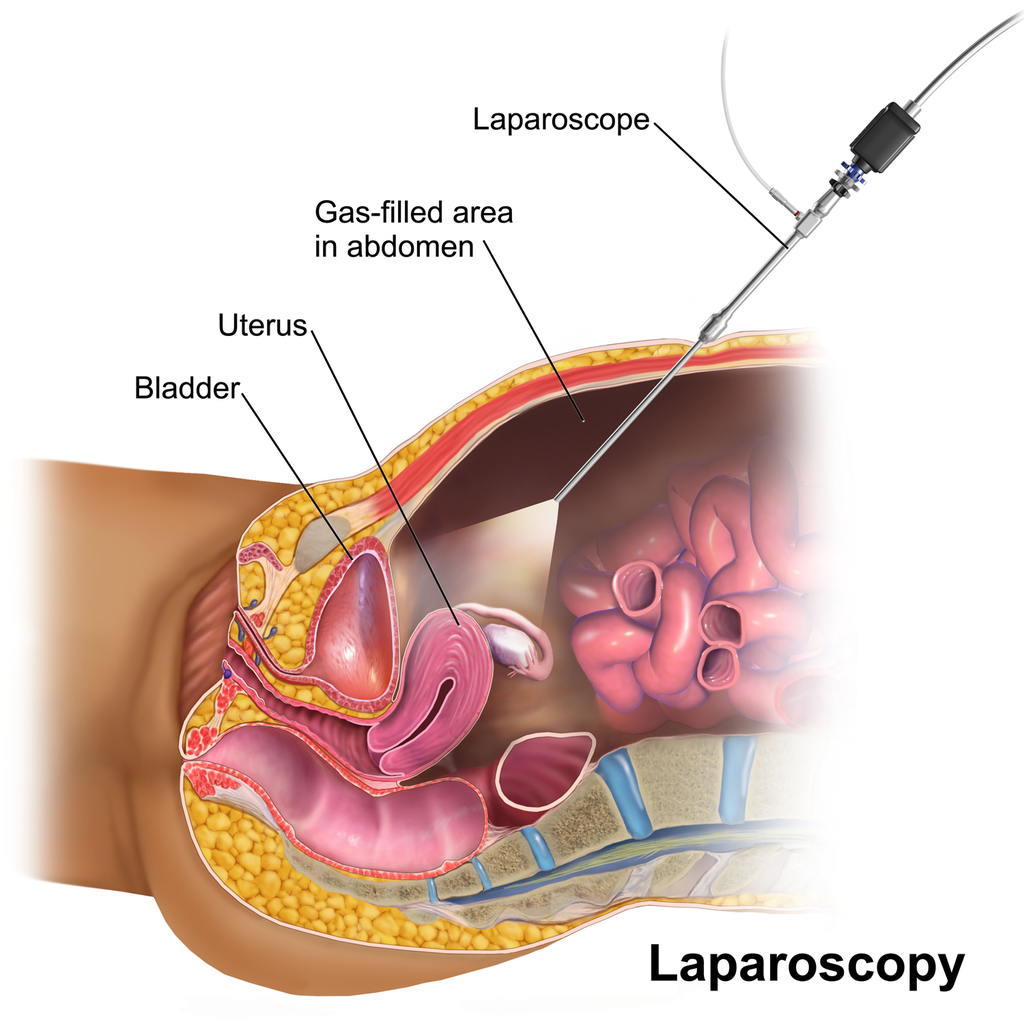
\includegraphics[width=0.45\textwidth]{images/laparoscopy_example_graphic.png}
\caption[Example MIS]{Illustration of MIS by Blausen et al.~\cite{laparosc_image2014blausen} The surgeon is getting the view of the operation scene by the laparoscope as real-time video.}
\label{img:laparoscopy}
\end{figure}

\begin{figure}
\centering
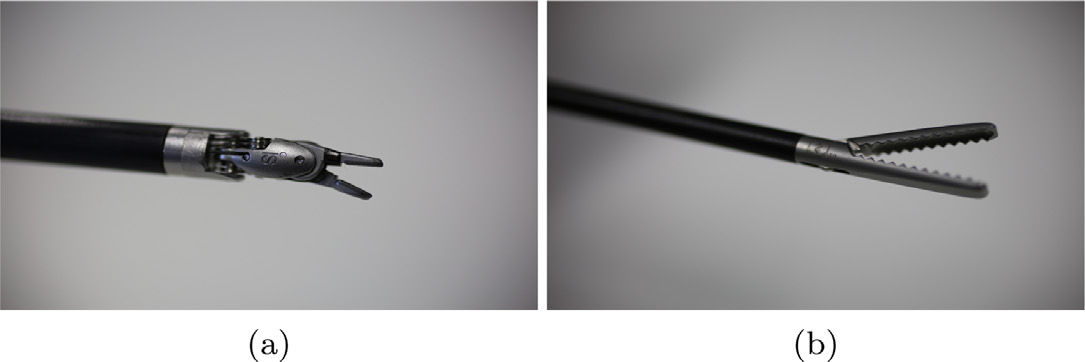
\includegraphics[width=0.5\textwidth]{images/laparoscopic_instruments.png}
\caption[Example MIS surgical instruments]{Examples of different MIS instruments: (a)~Da Vinci~\cite{da_vinci_localization2005Leven} articulated robotic instrument, (b)~rigid laparoscopic instrument~\cite{vision_based_surg_tool_det2017bouget}.}
\label{img:lap_instruments}
\end{figure}

Because the surgical instruments required for this technique are smaller and the advanced instrument 
design improves tissue manipulation, the surgical trauma for the patient after surgery is reduced~\cite{vision_based_surg_tool_det2017bouget}. 
Rutherford et al.~\cite{laparoscopic_adrenalectomy1996rutherford} showed in a laparoscopic adrenalectomy study that the postoperative inpatient stay was decreased from 9.8 to 5.1 days in comparison to the commonly known open surgery approach. Lacy et al.~\cite{laparoscp2002lacy} showed in a study regarding colorectoral cancer operation that patients treated with MIS recovered faster, had shorter hospital stays, and higher probability of cancer-related survival.

%\emph{Computer assisted intervention (CAI)} systems are used to gain information before and and during the surgery process with the aim to overcome these challenges.~\cite{vision_based_surg_tool_det2017bouget}

Before it is possible to perform MIS, the surgeons and the rest of the clinical team have to be trained to operate with MIS instruments. There are several challenges compared to open surgical approaches~\cite{haptic_feedback_surgery2009vanderMeijden}: 
The sense of touch for the surgeon is reduced and the view of the surgery is restricted by the endoscopic camera. It is also important to integrate image guidance to protect critical structures and help the surgeon to locate anatomical targets. Real-time knowledge of the position of the instruments within the surgical field of view is one of the main goals to improve MIS.~\cite{detect_instruments_mis2013allan} 

The following approaches are currently used to overcome the instrument localization challenge in MIS:
Electromagnetic tracking, which is realised by attaching an electromagnetic device to the instrument~\cite{electromagnetic_tracking2016lahanas}.
Optical localizers, where markers are applied to the surgical instrument and an additional external camera is used to recognize these markers and calculate the position of the instrument. This is the most widespread method in clinical use~\cite{optical_localizer_instr2010elfring}.
Other common methods are gaining positional information out of robotic surgery systems~\cite{da_vinci_localization2005Leven}, 
ultrasound-based methods~\cite{ultrasound_localization2009Hu}, and localization based on the endoscopic video used by the surgeon to operate~\cite{Laina2017}.

\section{Goals}
Image-based localization approaches are highly attractive because they do not require modification of the instrument design or the operating room, like for example electromagnetic tracking or optical localizers: 
The position and motion information is obtained directly from endoscopic camera used by the surgeon to operate. This is also the method with the lowest expenses.~\cite{vision_based_surg_tool_det2017bouget}
The aim is therefore to develop an image-based localization method for assistance and improvement of MIS.

% Input to proposed methods:
The input to the segmentation and localization methods proposed in this work are images out of an endoscopic video. The images contain surgical instruments.
%Def. Segmentation:
Segmentation means partitioning the input image into instrument part and background part. The partitioned image contains high pixel values where the instrument is located and low pixel values where the background is located.
% Def. Localization: 
Localization means extracting the pixel position of specific instrument landmarks out of the input image. In this work, the center point of the shown instruments is located.

Convolutional Neural Networks currently provide the best solutions for image segmentation~\cite{miccai15_results2018bodenstedt,long2015_FCNs}. This image segmentation task can be enhanced to localization of surgical instruments in images, as recently shown by Laina et al.~\cite{Laina2017}. 
In this work, the segmentation CNN proposed by Shvets et al.~\cite{Shvets2018} is extended with the aim to solve the localization task based on previously learned segmentation information.

%For the segmentation task, the prediction of the network divides the input image into instrument and background. The prediction is a greyscale image, where a high pixel value indicates a high probability that a part of the instrument is located at this position.  A low pixel value indicates a high probability that the background is shown at this pixel position. 
%
%For the localization task, the prediction of the network is a greyscale image that contains the highest pixel values near the instrument center point position.
%A low pixel value in the prediction indicates a high probability that this pixel is part of the background. In a postprocessing step, the exact position of the instrument is extracted out of the prediction image.
\chapter{Background}
\label{cha:background}

% Quelle für grundlegende Sachen:
% The content of this chapter is mainly based on the book ... proposed by .. et al. 

Convolutional Neural Networks have several advantages in image recognition in comparison to more conventional computer vision techniques~\cite{long2015_FCNs, imageNetWinner2012krizhevsky}.
They can be seen as an enhancement of Neural Networks. 

\section{Neural Network}
\label{nn:general}
A \emph{Neural Network~(NN)}~(see figure~\ref{draw:neural_network}) is an architecture that consists of a number of \emph{neurons}. These are interconnected in different ways and often organized into layers~\cite{neuralnetworks_old1994sarle}. 

\def\layersep{2.5cm}
\begin{figure}
\centering
\begin{tikzpicture}[shorten >=1pt,->,draw=black!50, node distance=\layersep]
    \tikzstyle{every pin edge}=[<-,shorten <=1pt]
    \tikzstyle{neuron}=[circle,fill=black!25,minimum size=17pt,inner sep=0pt]
    \tikzstyle{input neuron}=[neuron, fill=black!15!green];
    \tikzstyle{output neuron}=[neuron, fill=red!50];
    \tikzstyle{hidden neuron}=[neuron, fill=blue!60];
    \tikzstyle{annot} = [text width=4em, text centered]

    % Draw the input layer nodes
    \foreach \name / \y in {1,...,4}
    % This is the same as writing \foreach \name / \y in {1/1,2/2,3/3,4/4}
        \node[input neuron, pin=left:input {$x_\y$}] (I-\name) at (0,-\y) {};

    % Draw the hidden layer nodes
    \foreach \name / \y in {1,...,5}
        \path[yshift=0.5cm]
            node[hidden neuron] (H-\name) at (\layersep,-\y cm) {};

    % Draw the output layer node
    \node[output neuron,pin={[pin edge={->}]right:output}, right of=H-3] (O) {};

    % Connect every node in the input layer with every node in the
    % hidden layer.
    \foreach \source in {1,...,4}
        \foreach \dest in {1,...,5}
            \path (I-\source) edge (H-\dest);

    % Connect every node in the hidden layer with the output layer
    \foreach \source in {1,...,5}
        \path (H-\source) edge (O);

    % Annotate the layers
    \node[annot,above of=H-1, node distance=1cm] (hl) {hidden layer};
    \node[annot,left of=hl] {input layer};
    \node[annot,right of=hl] {output layer};
\end{tikzpicture}
% feedforward network??
\caption[Example structure Neural Network]{Example structure of a fully connected NN: Every circle denotes one neuron. This example network consists of three layers. The weights of the connections between the neurons are omitted in this figure.}
% reference somehow to http://www.texample.net/tikz/examples/neural-network/ where it's taken from.}
\label{draw:neural_network}
\end{figure}

One neuron consists of several \emph{inputs}~$x_i$, an \emph{activation function} $\alpha$ that processes these inputs, and one \emph{output~o}. % (see equation~\ref{eq:output_neuron}).

\begin{equation}
o = \alpha \left(\sum_{i=1}^n x_i \cdot w_i + b_k\right)
\label{eq:output_neuron}
\end{equation}

Every input value of a neuron is scaled by its corresponding \emph{weight} $w_i$.
The \emph{bias} $b_k$ influences the behaviour of the neuron by increasing or decreasing the sum of the scaled input values for the calculation of the output of the neuron.
The number of summands $n$ denotes the number of input values of the neuron.
%This output is defined by the so called activation function  that takes the input values scaled by the corresponding weights, and the bias value as parameters. The number of summands $n$ is the number of inputs of the neuron.

The specific output of the neuron depends on the kind of activation function $\alpha$:
Common activation functions are the sigmoid function (equation~\ref{eq:sigmoid_simple}) and the rectified linear unit (ReLU) (equation~\ref{eq:rectifier_fct}). The input of the activation function $\left( \sum_{i=1}^n x_i \cdot w_i + b_k\right)$ is abbreviated as $z$. % check if mathematically correct
% citations for equations needed
% maybe: insert graph of sigmoid, rectifier graph

\begin{equation}
\label{eq:sigmoid_simple}
sigmoid(z) = \frac{1}{1 + e^{-z}} = \frac{e^z}{e^z + 1}
\end{equation}

\begin{equation}
\label{eq:rectifier_fct}
rec(z) = z^+ = \max(0, z)
\end{equation}

For an example neuron structure with more detailed description see figure~\ref{draw:neuron}.

As the NN consists of many neurons, it consists also of the corresponding weights $w_i $ and biases $b_k$. The weights and biases are also referred to as \emph{parameters}.
The neurons of a NN are arranged into \emph{layers}.
These layers are distinguished into one input layer, hidden layers and one output layer.
In the network example in figure \ref{draw:neural_network}, the green layer is referred to as input layer, the red layer as output layer. The layers in between input and output layer, in the example one blue layer, are referred to as hidden layers. 
The network example is a \emph{Fully Connected Network (FCN)}: The output of each neuron in one layer is connected to each neuron in the following layer~\cite{long2015_FCNs}.

In this work, the calculation of the final output of the network with respect to its current weights and biases is denoted as $y_{w,b}(x)$. $x$ contains the input values to the network and can for example have vector or matrix shape.
% besser erklären: y "enthält" weights und biases?


% maybe citation unnecessary
% also abbreviate singular: NN, denote "network" as abbreviation of NN?

% maybe put weights more beautiful on arrow
% uncommented this because IT'S SO SLOW DURING COMPILATION
\begin{figure}
\centering
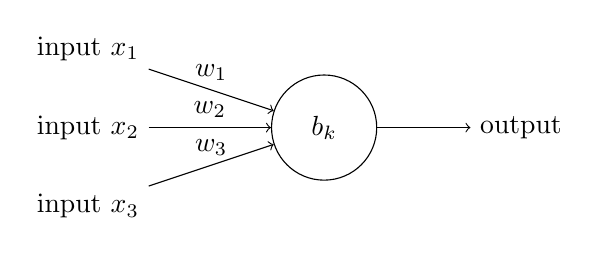
\begin{tikzpicture}
\path (0, 0) node[circle, draw, minimum size=38pt] (neuron) {$b_k$};
\path (-3, -1) node (arrow1start) {input $x_3$};
\path (-3, 0) node (arrow2start) {input $x_2$};
\path (-3, 1) node (arrow3start) {input $x_1$};
\path (2.5, 0) node (arrowfinalstart) {output};
\draw[->] (arrow1start) -- node[above] {$w_3$} (neuron);
\draw[->] (arrow2start) -- node[above] {$w_2$} (neuron);
\draw[->] (arrow3start) -- node[above] {$w_1$}(neuron);
\draw[->] (neuron) -- (arrowfinalstart);
\end{tikzpicture}
\caption[Example structure neuron]{General structure of a \emph{neuron}: The input values of the neuron are $x_1, x_2, x_3$. These input values are scaled by their corresponding weights $w_1, w_2, w_3$. $b_k$ denotes the bias. 
In this example, the output of the neuron using the sigmoid activation function is calculated by~$o={sigmoid\left(\sum_{i=1}^3 x_i \cdot w_i + b\right)}$.}
\label{draw:neuron}
\end{figure}

\subsection{Training Data}
\label{nn:training_data}
%The proposed training method in this work belongs to the \emph{supervised} learning methods, because the desired output of the network is known during the training process % When training a NN with data where the corresponding ground truth is unknown, the training procedure belongs to the \emph{unsupervised} learning methods. -> zu ausführlich, unsupervised weglassen
\emph{Training data} is used for the training process (see section~\ref{nn:training_methods}) of a NN. This training data is often composed of several datasets, later referred to as \emph{training sets}. One training set $\{(x_1,t_1),...,(x_j,t_j),...,(x_N,t_N)\}$ contains $N$ \emph{training samples} $(x_j,t_j)$ with one \emph{training input}~$x_j$ and the corresponding \emph{target $t_j$}.

The input given to the NN is denoted as $x_j$. The desired output of the network for the corresponding $x_j$ is $t_j$. The target $t_j$ is also referred to as \emph{ground truth} or \emph{label}. 
Since for each input $x_j$ the corresponding ground truth $t_j$ is known, this is referred to as a \emph{supervised} machine learning problem.

When there is little training data available, the network can not be trained sufficiently to predict the desired output. % insert citation here
The approach to train the network for many iterations with the same, small training dataset can cause overfitting (see section~\ref{nn:testing}).
To avoid this problem, a commonly used method is \emph{data augmentation}: The dataset is artificially enlarged by operations on the different training samples $(x_j,t_j)$. Commonly used transformations are, given that the input of the network are images, translation~\cite{augmentation_SAR2016Ding}, horizontal and vertical reflections, and altering the RGB channels of the images.~\cite{imageNetWinner2012krizhevsky}

\subsection{Network Training}
\label{nn:training_methods} % maybe another heading  
The general aim of training a NN is that, after the training is finished, the network recognizes certain features of the input data and classifies the input accordingly. These features are learned by each weight $w_i$ and each bias $b_k$ of the network during the training phase.
% With this information learned during training, the NN is capable of predicting several \emph{classes} out of the given input. These classes are specified in the ground truth of the training set. ---> weglassen weil sonst classification problem erklären 
The resulting network out of a network structure that learned specific parameters is referred to as \emph{model}. 

The prediction result of a NN with given input $x$ is calculated as $y_{w,b}(x)$.
During the training period, the deviation between $y_{w,b}(x_j)$ for the training input $x_j$ and the corresponding desired output $t_j$ is calculated and referred to as error $E_j$.
The aim is to adjust the parameters of the network in a way that $E_j$ is minimized.

% loss function: decides how to calculate the difference between output and desired output
The \emph{loss function} $L(y_{w,b}(x_j), t_j)$ of the NN specifies the way how $E_j$ is determined for one training sample $(x_j,t_j)$.
The loss function is also often referred to as cost function. 
% The function $y_{w,b}(x_j)$ calculates the output of the network respective to its current weights and biases, given the input $x$. -> maybe to much detail

One of the most common loss functions is the mean squared error (MSE):
\begin{equation}
MSE(y_{w,b}(x_j), t_j) = (t_j-y_{w,b}(x_j))^2
\label{eq:mean_sq_error}
\end{equation}

As the loss $L(x_j,t_j)$ is calculated for each training sample , the results are summed and then averaged over the complete training set $\{(x_1,t_1),...,(x_j,t_j),...,(x_N,t_N)\}$. This calculation of the overall error $E$ is stated in equation~\ref{eq:mean_loss_all_inputs} for $N$ training inputs.

\begin{equation}
E = \frac{1}{N} \sum_{j=1}^N L(y_{w,b}(x_j), t_j)
\label{eq:mean_loss_all_inputs}
\end{equation}

$E$ is reduced by adjusting the weights and biases of the network with the \emph{gradient descent} method~\cite{backprop_grad_desc_closed1993shun}. 
To reduce $E$, the partial derivatives of the loss function with respect to all $G$ weights $w_i$ and all $D$ biases $b_k$ of the network are calculated stepwise.
Afterwards, each weight $w_i$ and each bias $b_k$ in $y_{w,b}(x_j)$ is adjusted.
%The loss function is derivated partially by weights and biases that are part of the parameter $y_{w,b}(x_j)$. 
The partial derivatives are contained in two \emph{gradients} of the loss function: $\nabla E_{w}$ for the weights and $\nabla E_{b}$ for the biases of the network.

\begin{equation}
\nabla E_{w} = \left(\frac{\partial E}{\partial w_1} , ... ,\frac{\partial E}{\partial w_i}, ... , \frac{\partial E}{\partial w_G}\right)^T
\label{eq:gradient_weights}
\end{equation}

\begin{equation}
\nabla E_{b} = \left(\frac{\partial E}{\partial b_1} , ... , \frac{\partial E}{\partial b_k}, ... , \frac{\partial E}{\partial b_D}\right)^T
\label{eq:gradient_biases}
\end{equation}

Every weight $w_i$ and every bias $b_k$ in the loss function is updated to $w'_i$ and $b'_k$ by using the entries of $\nabla E_{w}$ and $\nabla E_{b}$.

\begin{equation}
w'_i = w_i - \lambda \frac{\partial E}{\partial w_i} 
\label{eq:update_weight} 
\end{equation}

\begin{equation}
b'_k = b_k - \lambda \frac{\partial E}{\partial b_k}  
\label{eq:update_bias}
\end{equation}

The parameter $\lambda$ refers to the \emph{learning rate}. It is used to control the learning process of the network by scaling the adjustment of the weights and biases. % citation needed -> include general book that explains this at beginning
% maybe include word "update rule"

The gradients $\nabla E_{w}$ with $G$ entries and $\nabla E_{b}$ with $D$ entries are summarized into one gradient $\nabla E$. 

\begin{equation}
\nabla E = \left(\frac{\partial E}{\partial w_1},..., \frac{\partial E}{\partial w_i}, ... ,\frac{\partial E}{\partial w_G},\frac{\partial E}{\partial b_1}, ..., \frac{\partial E}{\partial b_k}, ..., \frac{\partial E}{\partial b_D}\right)^T
\label{eq:nabla_L}
\end{equation}

Each entry $\frac{\partial E}{\partial w_i}$ and $\frac{\partial E}{\partial b_k}$ of $\nabla E$ is calculated separately for every training sample $(x_j,t_j)$, and then averaged over all $N$ training samples.

\begin{equation}
\nabla E = \frac{1}{N} \sum_{j=1}^{N} \nabla E_j
\label{eq:mean_nabla_L}
\end{equation}

Calculating the gradient over all the training samples and afterwards averaging the result is computationally expensive. 
To reduce the learning time of the network, it is common to use a modified gradient descent method: It is denoted as \emph{stochastic gradient descent}. % maybe cite here  
The gradient $\nabla E$ is estimated by calculating the gradient for a subset of $\beta$ samples out of the training set, and then averaging the result: $\frac{1}{\beta} \sum_{i=1}^\beta \nabla E_i$.
The subset of the original training set is referred to as \emph{mini-batch}. The number of elements of the mini-batch, $\beta$, is the \emph{batch size}. Training the NN with randomly picked mini-batches also has the advantage of avoiding shifts of the network.~\cite{batch_normaliz2015ioffe}
When the complete training dataset was shown to the network, i.e. every element of the training dataset was propagated through the network one time, one \emph{epoch} of training is completed.

% not sure if this backprop description is correct:
\emph{Backpropagation~(BP)}~\cite{rumelhart1986origin_backprop_paper} is one way to efficiently calculate all partial derivatives of the network~\cite{backprop_grad_desc_closed1993shun}.
It is by far the most common approach for training NNs~\cite{hernandez_adams2015prob_backprop}.
First, the forward pass of the training phase is performed: The output of the NN is calculated out of the given input.
The gradients $\nabla E_j$ are calculated for each input of the mini-batch by backpropagating the error $E_j=L(y_{w,b}(x_j), t_j)$ back through the network. Then, the update step is performed: Every weight $w_i$ and bias $b_k$ of the network is corrected according to the calculated gradients.~\cite{rumelhart1986origin_backprop_paper}~\cite{buscema1998backprop_network}  

\subsection{Network Testing}
\label{nn:testing}

%% generalization error 
When training a NN, the aim is to obtain a network with optimal generalization performance. Generalization performance means that $E$ is minimal on network inputs not seen during training. This $E$ is also referred to as \emph{generalization error}.~\cite{cross_val_overfit1998prechelt}

Therefore, when testing the performance of a NN, it is necessary to provide input that was not given to the network during the training procedure. These previously unseen input data is referred to as \emph{test data}.
This test data is composed of several \emph{test sets}. One test set $\{(\mathbf{x_1},\mathbf{t_1}),...,(\mathbf{x_l},\mathbf{t_l}),...,(\mathbf{x_M},\mathbf{t_M})\}$ consists of $M$ \emph{test samples} $(\mathbf{x_l},\mathbf{t_l})$ with one test input $\mathbf{x_l}$ and its corresponding target $\mathbf{t_l}$.

When the generalization error increases during training, this indicates a problem that is denoted as \emph{overfitting}: While the network seems to get better and better during training, i.e. $E$ on the training dataset decreases, the network actually begins to predict worse on the test set, the generalization error increases.~\cite{cross_val_overfit1998prechelt}
The prediction performance of the network is fitted to the training dataset, but generalizes poorly.

It is a commonly used method to split the given data into separated training and testing sets and evaluate the network with the \emph{cross-validation} method. 

In \emph{k-fold cross-validation}, all training data is assigned randomly to $k$ datasets with approximately the same size. These $k$ datasets are separated into $k-1$ training sets and in one remaining test set. 
The NN is trained on the $k-1$ training sets and then evaluated on the remaining test set. This procedure is done $k$ times. Each time another set is chosen as test set, consequently the training sets are also different each time. As a result, there are $k$ different models of the NN. The performance of the NN is evaluated by testing each model on its corresponding test set and averaging the results over all models.

Another variant of k-fold cross-validation is \emph{leave-one-out cross-validation (LOOCV)}: 
For the given training data with $N$ elements, one sample $(\mathbf{x_l},\mathbf{t_l})$ is chosen as test sample, the rest of the data as training samples. Every element is chosen once as a test sample. The performance of the resulting models is evaluated the same way as for k-fold cross-validation, with $k=N$.

Cross-validation is a useful method to estimate the generalization error: The evaluation of the network includes all available labeled data without having used it for training and testing at the same time.~\cite{loocv_prev_overfit1997Ng} 

%%% pre-trained 
A NN structure which has already adjusted weights and biases due to previous training on several datasets, for example ImageNet~\cite{pre_trained_overfit2016marmanis}, is also referred to as \emph{pre-trained} network.
%When solving tasks like for example image recognition by using pre-trained networks, $E$ is reduced in comparison to using randomly initialized networks for the task~\cite{imageNetWinner2012krizhevsky}.
%The problem of overfitting is reduced by using a pre-trained network, especially when there are few training data available.~\cite{pre_trained_overfit2016marmanis} -> correction to:
Using pre-trained networks instead of randomly initialized networks to solve tasks such as image recognition reduces both $E$
and overfitting, especially when there are few training examples available\cite{imageNetWinner2012krizhevsky, pre_trained_overfit2016marmanis}.

\section{Convolutional Neural Network}
\label{cnn:general}
A \emph{Convolutional Neural Network (CNN)} is a specific kind of NN. The first application of CNNs was developed by LeCun et al.~\cite{first_cnn1998lecun}. In the following, the structure of a CNN is explained, given that it is used for image recognition.

% input image == values of first "feature map"
% Input of a CNN: Matrix with three dimensions -> 2 dimensions are image resolution 
In this scenario, the input to a CNN consists of an image with three dimensions. For example a RGB image has two dimensions for the resolution and one dimension for the RGB channels. This input is referred to as \emph{input layer}, the dimensions as \emph{channels}.

%One layer consists of several \emph{feature maps} (?)
% "spatial dimensions": first 2 dimensions / height, width
One CNN consists of multiple \emph{feature maps}, see for example U-Net in figure~\ref{img:basic_u-net}.
These feature maps usually have three dimensions: Two spatial dimensions for width and height, and a third dimension which denotes the number of channels. The input image is also a feature map.

Convolutions with a specific kernel size are applied to the feature maps, followed by an activation function $\alpha$ (see section~\ref{nn:general}). The result of the convolutions is stored in the following feature map of the CNN. The kernel is also referred to as \emph{filter}.
In a CNN structure, the parameters of the neurons are not realized with direct connections between neurons like in a general NN: They are stored in the filters of the CNN.
The learning process with gradient descent works like for NNs in general, but in particular the weights of the filters of the CNN are updated.

The number of feature map dimensions and filter dimensions is always the same.
The first two dimensions of the filter are applied to the spatial dimensions of the feature map. These dimensions of the filter are usually smaller than the corresponding feature map dimensions it is applied to. 
% The width and height of the kernel are smaller than the feature map is is applied to.
The third dimension of the filter always has the same size as the number of channels of its input feature map. This means that the filter extends through the full depth of its input volume.~\cite{lecun1990handwritten_digit_recog} 
The \emph{stride} of a filter denotes the distance between the regions of the feature map it is applied to.

The state-of-the-art CNNs, especially for image segmentation, consist of one \emph{downsampling phase} followed by an \emph{upsampling phase}. These are also denoted as \emph{encoder} and \emph{decoder} of the network.
In the downsampling phase, the input of the network is reduced stepwise by convolutions. % at the same time the number of feature maps is increased. 
In the upsampling phase, the size of the output after the downsampling phase is increased again by application of deconvolutions.~\cite{Shvets2018, du2018_2D_pose_est_CNN} 
U-Net~(see figure~\ref{img:basic_u-net}) proposed by Ronneberger et al.~\cite{Ronneberger2015} is a typical encoder-decoder CNN used for segmentation of images (see figure~\ref{img:basic_u-net}). 

\begin{figure}
	\centering
	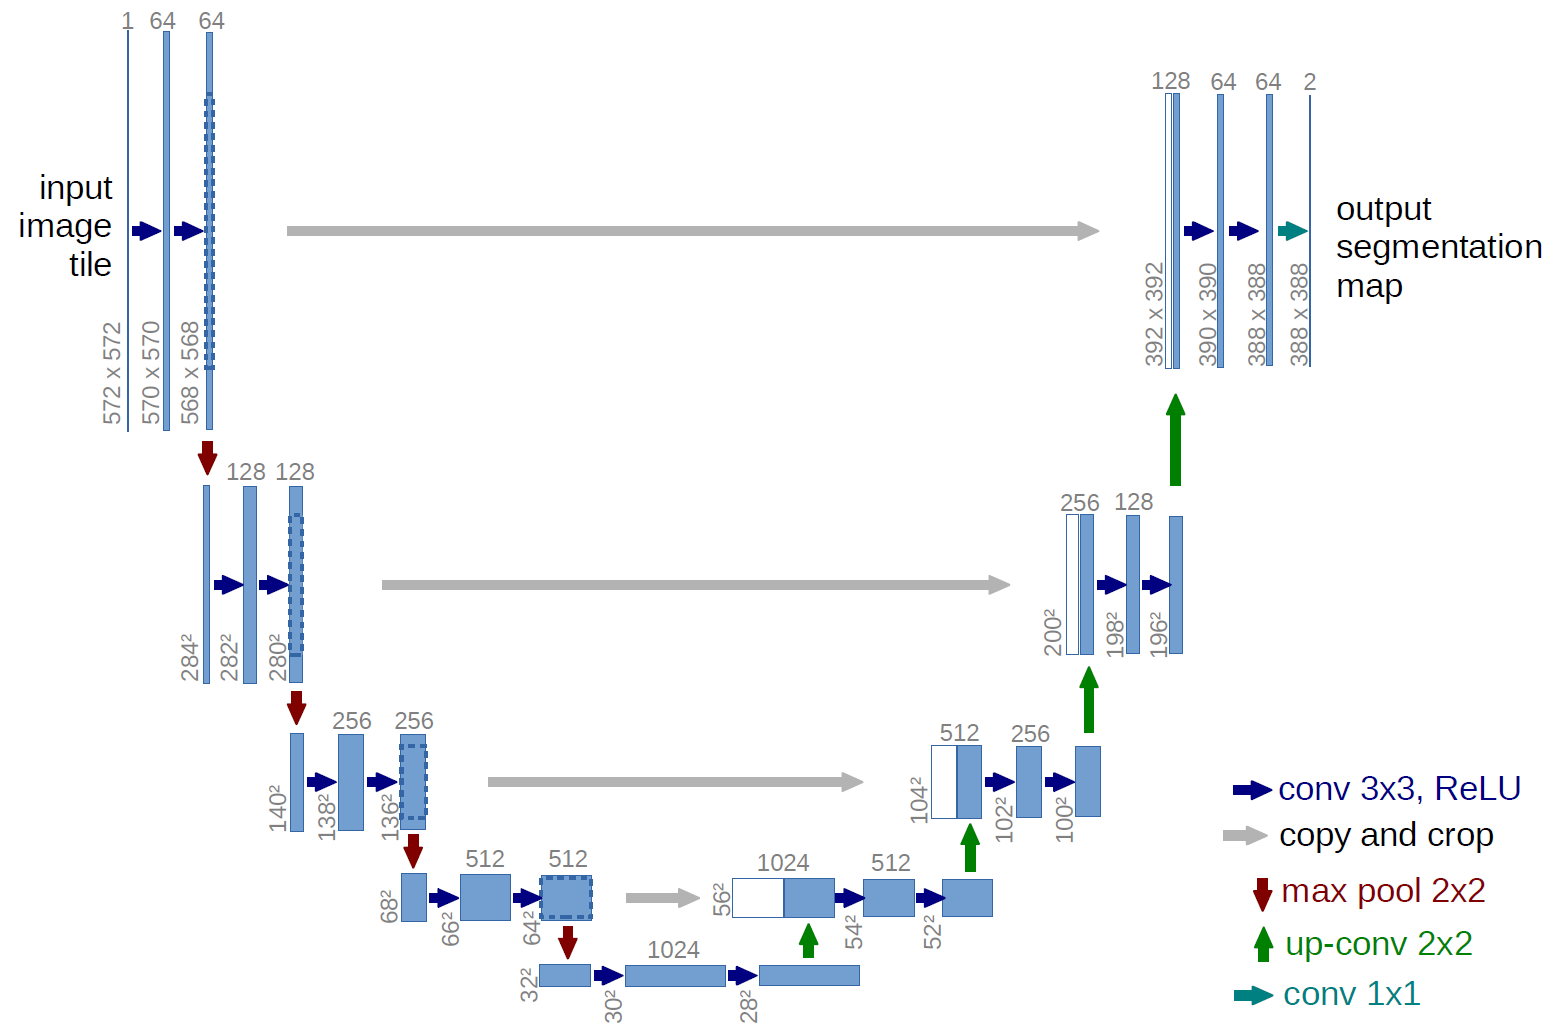
\includegraphics[width=.7\textwidth]{images/networks/u-net-architecture.png}
	\caption[Structure of U-Net]{Structure of U-Net, proposed by Ronneberger et al.~\cite{Ronneberger2015}. Each blue box corresponds to a multi-channel feature map. The number of channels is denoted on top, the resolution of the map is denoted at the left side of the box. White boxes refer to feature maps that are copied from the encoder phase and concatenated to the decoder phase. The arrows denote the operation types of the network.}
	\label{img:basic_u-net}
\end{figure}

There exist different kinds of convolutions. In the encoder phase of the network, the applied convolutions mostly preserve or reduce the spatial dimensions of the input and increase the number of channels. 
In the decoder phase, the convolutions mostly preserve or increase the spatial dimensions of the input and decrease the number of channels. This type of convolution is referred to as \emph{transposed convolution}, \emph{deconvolution} or \emph{upconvolution}. To increase the spatial dimensions, \emph{padding} is included for the convolutions.
% give example pic for convolution / cite convolution

\emph{Pooling} in CNNs is realized by a filter that reduces the dimension of its input. It is a widely used method to downsample the feature maps in the encoder phase of the network. The most common pooling method is \emph{max pooling}: Only the maximum value of the input region of the filter is returned.

% optimizer

% explain RNN -> needs reference in State of the Art

% explain ex vivo (refer here from methods / explain in methods)
% explain morphology opening (refer here from methods / explain in methods)

%\subsection{Fully Convolutional Network} ->this is not really correct
%\label{sec:FCN}
% explain FCN -->Fully Convolutional Networks (FCN) are a particular type of CNN recently proposed by \cite{long2015_FCNs} out of \cite{garcia2017segm_nonrigid_book}, reference to "fully connected" explanation in NN -> isn't explained yet
%A widely used architecture for CNNs are Fully Convolutional Network (FCN). The basic operations like convolutions, pooling and activation functions operate on local receptive fields. In FCNs, these operations are applied completely to their input. The feature maps of a FCN are referred to as \emph{fully connected layers}.~\cite{long2015_FCNs}


\chapter{State of the Art}
\label{cha:stateOfTheArt}
% The following works propose state-of-the-art methods to get the localization of surgical instruments during MIS.
% feature map -> used in State of the Art. search here and reference to bg
The following works propose current state-of-the-art solutions for surgical instrument segmentation and localization in endoscopic videos.

% better description of this paper / abbreviations of submitted CNNs / teams
% explain better difference between merged method and "single" method

%%%%%%%%% Comparative evaluation of instrument segmentation and tracking methods in minimally invasive surgery %%%%%%%%%
 
Bodenstedt et al.~\cite{miccai15_results2018bodenstedt} present the results of the methods submitted for EndoVis15 (see section~\ref{sec:endovis15}). Additionally, they propose merged results from the submitted models because it significantly increases accuracy in comparison to the best submitted stand-alone method. These results show that the CNN-based methods reached the highest performance compared to other methods. Therefore, in the following part of this chapter, only CNN-based methods concerning image-based segmentation of surgical instruments will be described.
% SEG-KIT-CNN
For EndoVis15-S, SEG-KIT-CNN is proposed: It is a FCN that uses VGG-16~\cite{simonyan2014vgg} as an encoder.

%%%%%%%%% Real-Time Segmentation of Non-rigid Surgical Tools Based on Deep Learning and Tracking %%%%%%%%%
Garcia et al.~\cite{garcia2017segm_nonrigid_book} propose two adapted FCNs for EndoVis15-S: FCN and FCN-real-time.
The forward evaluation takes 100ms for the FCN which is below the frame rate of an endoscopic video. The frame rate of an endoscopic video is usually 25 frames per second (fps), 30~fps or 60~fps.
% explanation not soo good
The FCN-real-time approach overcomes this problem by estimating an affine transformation on the instrument between the time of two segmentations of the network. 
When a frame is read from the surgical video feed, it is sent to the FCN-real-time only if the network is not busy processing the previous frame.

%%%%%%%%% Deep Residual Learning for Instrument Segmentation on Robotic Surgery %%%%%%%%%
Pakhmov et al.~\cite{deep_residual_instr_segm2017pakhmov} propose a ResNet-101 which is converted into a FCN for EndoVis15-S (ResNet-FCN).

%%%%%%%%% Surgical tool segmentation using a hybrid deep CNN-RNN auto encoder-decoder %%%%%%%%%
% in picture of network: take rigid set but results are for robotic ?? ok.
% include ref for recurrent network!
Attia et al.~\cite{Attia2017_surg_tool_cnn-rnn} provide a Convolutional Neural Network - Recurrent Neural Network (hybrid CNN-RNN) auto encoder-decoder network~(see figure~\ref{img:hybrid_cnn_rnn}) for instrument segmentation for EndoVis15-S.

\begin{figure}
	\centering
	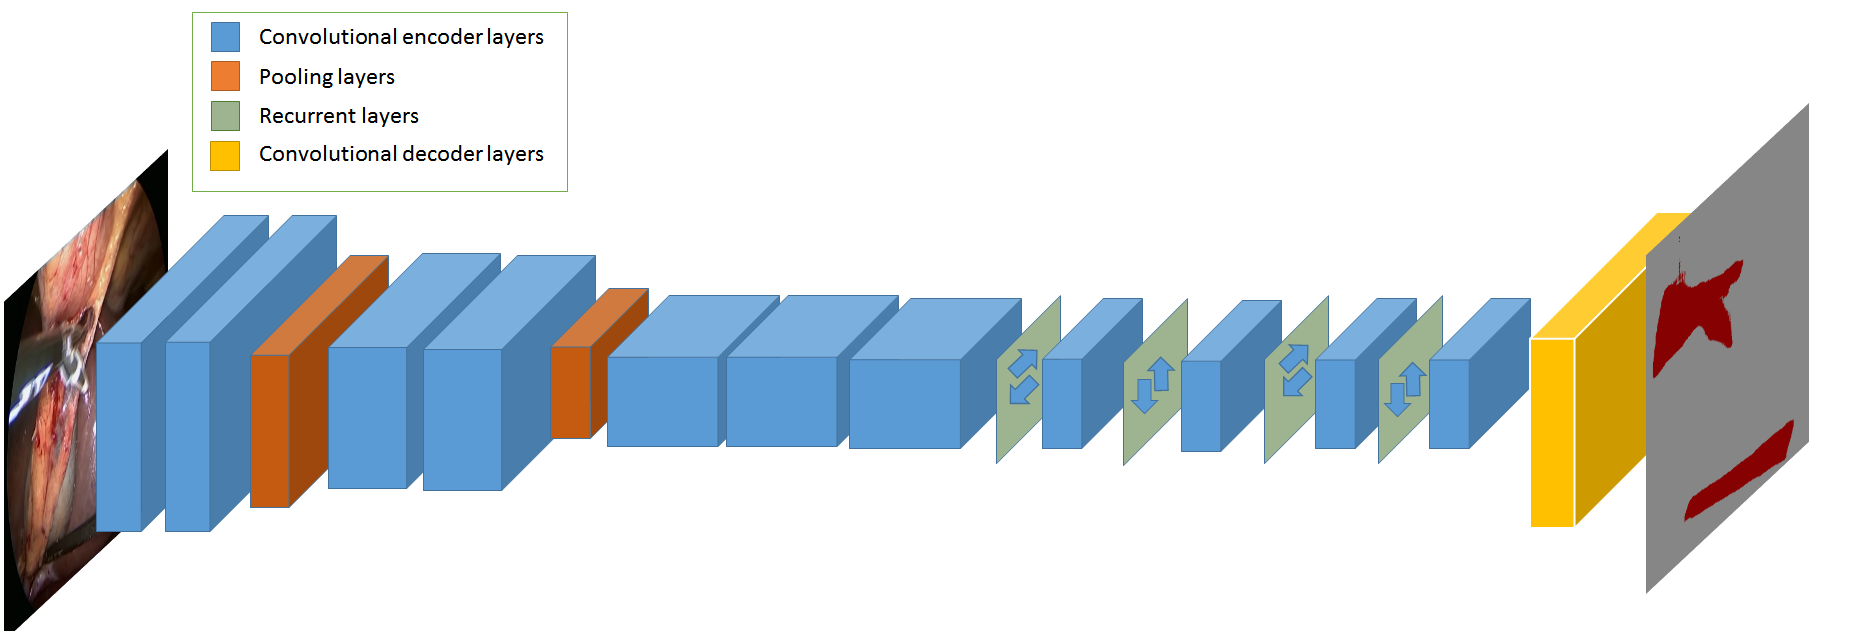
\includegraphics[width=.8\textwidth]{images/networks/hybrid_cnn_rnn.png}
	\caption[CNN-RNN architecture~\cite{Attia2017_surg_tool_cnn-rnn}]{Proposed hybrid CNN-RNN architecture by Attia et al.~\cite{Attia2017_surg_tool_cnn-rnn}.
	The encoder phase of the network consists of seven convolutional layers denoted as blue blocks, 
	the two max-pooling layers are denoted as orange blocks. 
	The feature maps extracted by the encoder part of the network are fed into 4 layers of the recurrent network, denoted as green masks
	with 4 decoupled directions. The output mask of the instrument is reconstructed using an auto decoder network, denoted with yellow blocks.}
	\label{img:hybrid_cnn_rnn}
\end{figure}

%%%%%%%%% Concurrent Segmentation and Localization for Tracking of Surgical Instruments %%%%%%%%%
Laina et al.~\cite{Laina2017} propose three different CNN-based approaches to predict the location of surgical instruments (see figure~\ref{img:csl_network}).
They are abbreviated as L-network, SL-network and CSL-network. 
All of the proposed networks share ResNet-50~\cite{deep_res_learning_img_rec2016He} as encoder part.

The decoder part of the L-network regresses the positions of the instrument directly as a 2x$n_i$ dimensional vector, where $n_i$ is one predicted location of one instrument. This method is frequently used in literature.~\cite{landmark_localization_2Dvector2016rupprecht}
The segmentation task of the instrument is excluded in this approach.

In the SL-network, the prediction of the 2D locations of the instrument and the segmentation of the instrument are combined in one architecture. 
Both tasks share weights along the encoder part and split into two distinct parts at the decoder part of the network. The prediction of the instrument positions is solved like in the L-model.
For the segmentation task, the probability of each pixel of belonging to the instrument or the background is predicted.

The CSL-network predicts the position of the instrument by regressing a heatmap instead of the exact coordinates.
The heatmap for training is created by applying a two-dimensional Gaussian function to the ground truth position of the instrument (see section~\ref{sec:heatmaps}). 
By applying this method, the problem that ground truth annotations of the instrument position
can differ by several pixels is avoided. The segmentation and localization task share weights over the entire network because the heatmaps have the same size as the segmentation masks.
The CSL-network outperforms the two other proposed methods.

\begin{figure}
	\centering
	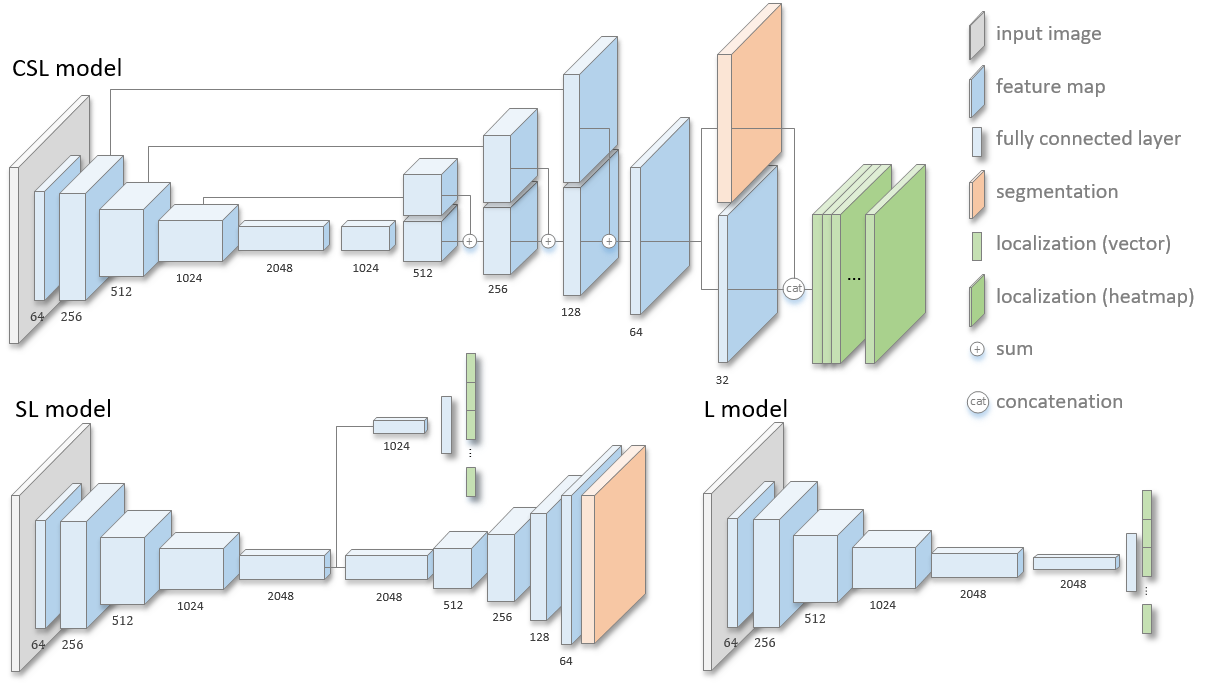
\includegraphics[width=.6\textwidth]{images/networks/CSL_network.png}
	\caption[Concurrent Segmentation and Tracking Networks~\cite{Laina2017}]{The three proposed network architektures in Laina et al.~\cite{Laina2017}}
	\label{img:csl_network}
\end{figure}

%%%%%%%%% Articulated Multi-Instrument 2-D Pose Estimation Using Fully Convolutional Networks %%%%%%%%%%%
% too complicated maybe
Du et al.~\cite{du2018_2D_pose_est_CNN} solved the localization task by using a fully convolutional detection-regression network (FCN-det-reg) (see figure~\ref{detection-regression-net}), where the instrument joints and associations between joint pairs are located by the detection subnetwork and subsequently redefined by the regression subnetwork. 

\begin{figure}
	\centering
	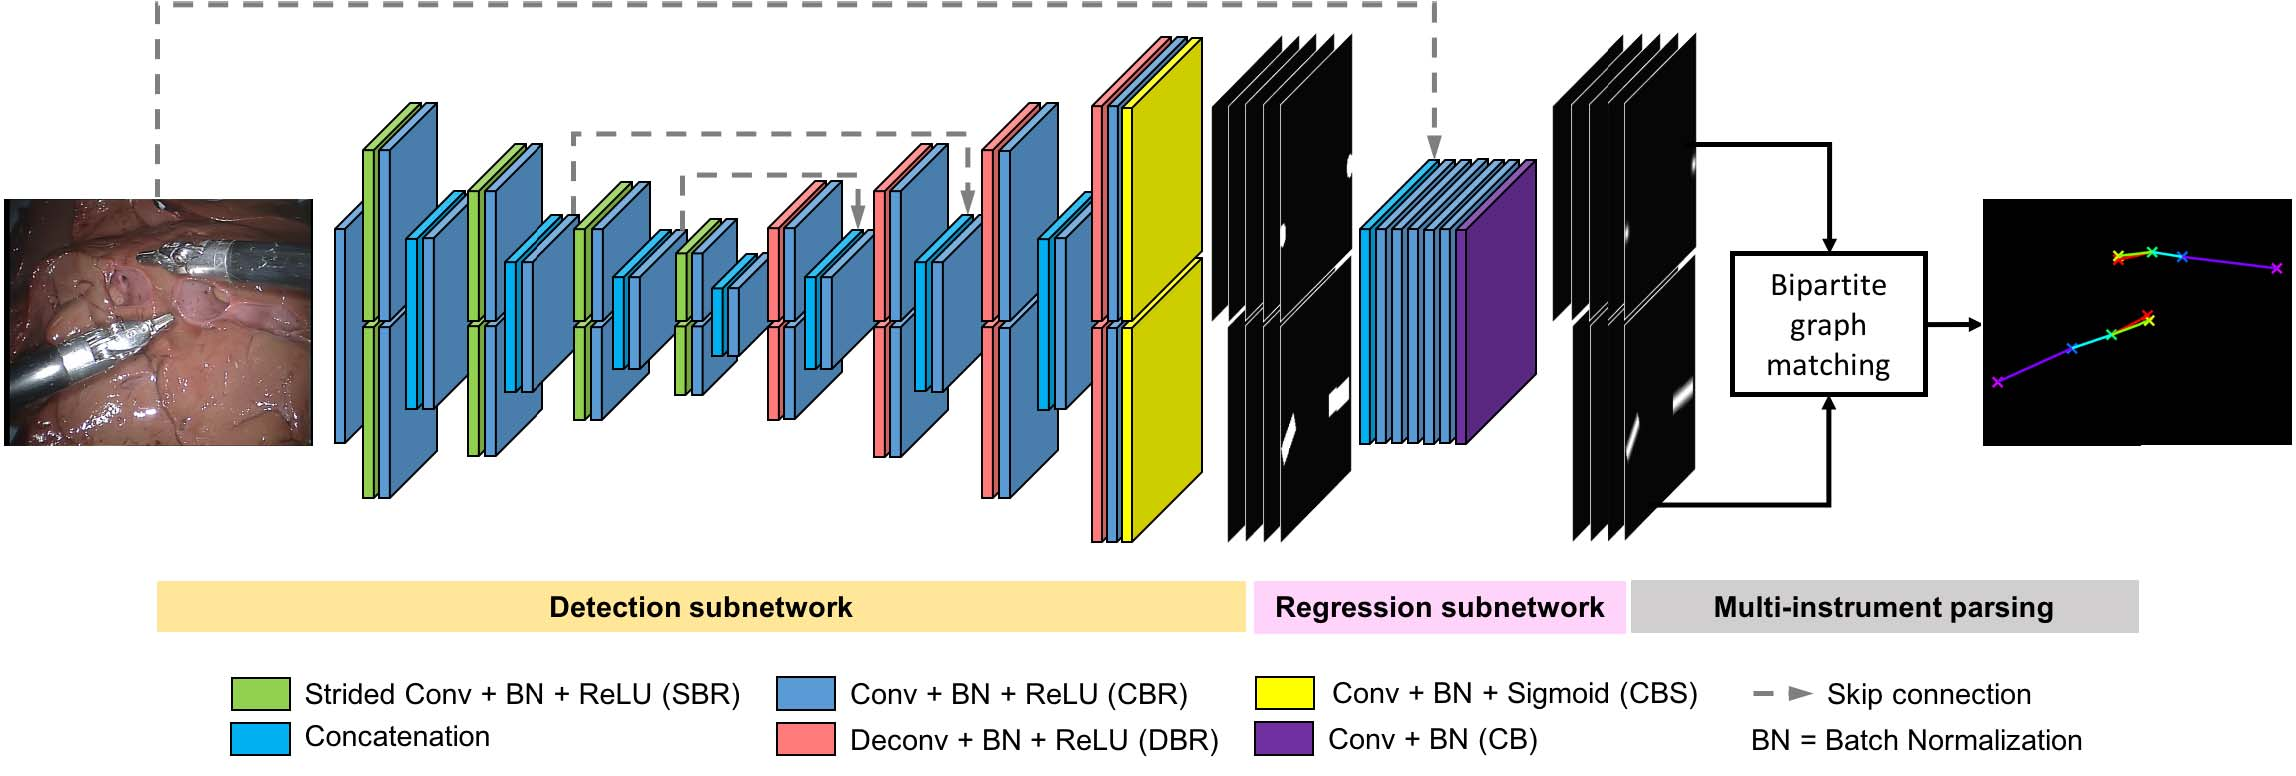
\includegraphics[width=.8\textwidth]{images/networks/detection-regression.jpg}
 	\caption[Detection-regression network~\cite{du2018_2D_pose_est_CNN}]{Structure of the detection-regression network proposed in Du et al.~\cite{du2018_2D_pose_est_CNN}}
 	\label{detection-regression-net}
\end{figure}

Positions of the surgical instruments are inferred using maximum bipartite graph matching~\cite{bipartite_graph2005schwartz}.
The EndoVis15-T (see section~\ref{sec:endovis15}) ground truth annotations were modified and replaced by self-generated annotations (see figure~\ref{modified_gt_2D_pose}).

\begin{figure}
\centering
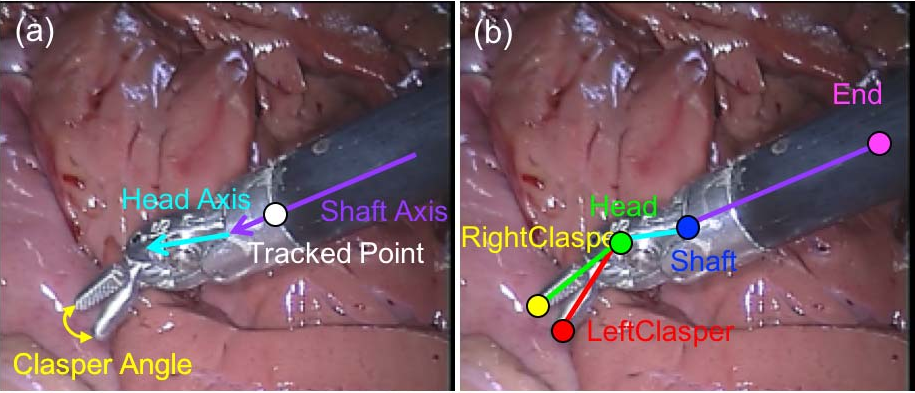
\includegraphics[width=.6\textwidth]{images/dataset/annotated_gt.png}
\caption[Modified ground truth annotation~\cite{du2018_2D_pose_est_CNN}]{The original (a) and modified (b) ground truth annotations for EndoVis15-T.}
\label{modified_gt_2D_pose}
\end{figure}

The detection part of the network (see figure~\ref{detection-regression-net}) consists of two branches. 
The first branch is used to predict probability maps for each joint of the surgical instrument, 
the second branch is used to predict association probability maps for each joint pair.
% Therefore, the ground truth for the detection subnetwork is constructed as a set of the joint and joint pair binary maps (see figure~\ref{img:gt_association_binary_joint}). -> unnecessary, delete pic
From the prediction of the detection part, a coarse position of the instrument is obtained. With the regression part of the network, that takes the prediction of the detection part as an input, refined positions of the joints are obtained.
The ground truth for the regression subnetwork for each instrument joint location consists of heatmaps formed by a two-dimensional Gaussian distribution at the labeled position of the joint. 
The ground truth for the association between joint pairs are formed by a Gaussian distribution along the joint pair center line.
The approach to use heatmaps in form of images to predict the instrument position is similar to Laina et al.~\cite{Laina2017}.

Notably, it is not possible to compare the FCN-det-reg results directly to the other results: The provided ground truth is modified, the results that exceed a certain threshold are excluded from evaluation, and the training procedure is different from the challenge guidelines.

% Notably, the network is trained with the entire training data instead of a LOSO training strategy as specified by the EndoVis15 challenge guidelines (see section~\ref{sec:endovis15_robotic_test}). 
% That makes the results incomparable to the results that are obtained by other solutions trained accordingly to the challenge guidelines.

%%%%%%%%%%  Simultaneous Recognition and Pose Estimation of Instruments in Minimally Invasive Surgery %%%%%%%%% 
%Kurmann et al.~\cite{kurmann2017sim_recogn_pose_estim} propose a modified U-Net architecture (see figure~\ref{img:kurmann_u_net_multi_instr}) to detect multiple instrument positions.
%The results are calculated
%
%\begin{figure}
%	\centering
%	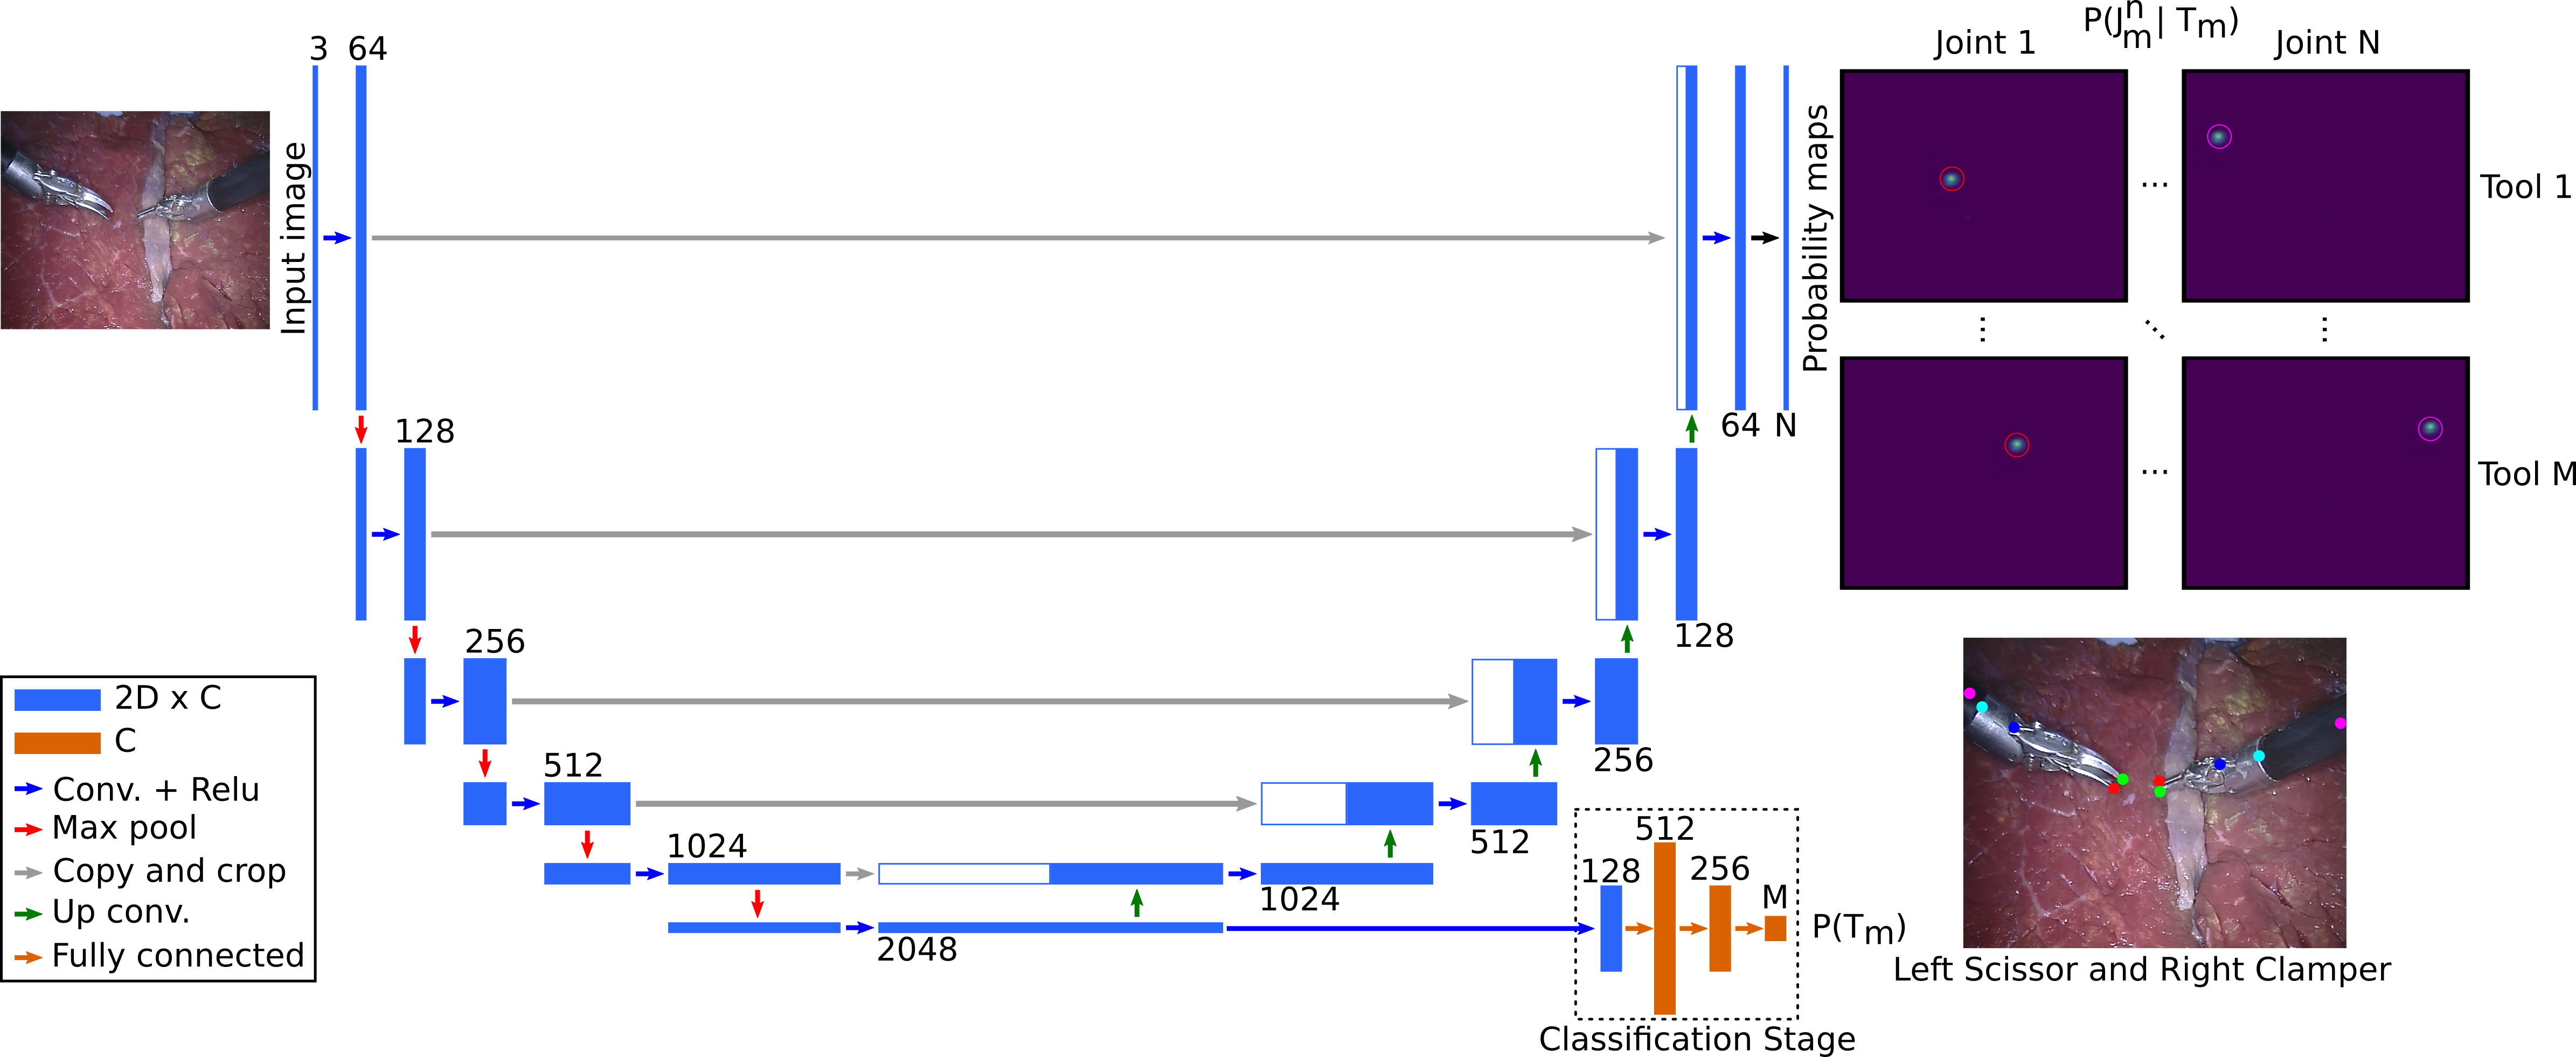
\includegraphics[width=.7\textwidth]{images/networks/multi_instr_u-net.png}
%	\caption{U-Net based multi-instrument detector network architecture proposed by Kurmann et al.~\cite{kurmann2017sim_recogn_pose_estim}}
%	\label{img:kurmann_u_net_multi_instr}
%\end{figure}

%%%%%%%%% Automatic Instrument Segmentation in Robot-Assisted Surgery Using Deep Learning %%%%%%%%%
Shvets et al.~\cite{Shvets2018} used four different networks for EndoVis17-S (see section\ref{sec:endovis17}):
U-Net (see figure~\ref{img:basic_u-net}), TernausNet-11 and TernausNet-16 which are a modifications of U-Net, and one network that is a modification of LinkNet~\cite{linknet2017Chaurasia}.
TernausNet-16~(see also figure~\ref{img:ternausnet16}) outperforms the other networks in the segmentation tasks except for the inference time.
VGG16~\cite{simonyan2014vgg}, pre-trained (see section~\ref{nn:testing}) on ImageNet, is used as encoder  for TernausNet-16.

\begin{figure}
	\centering
	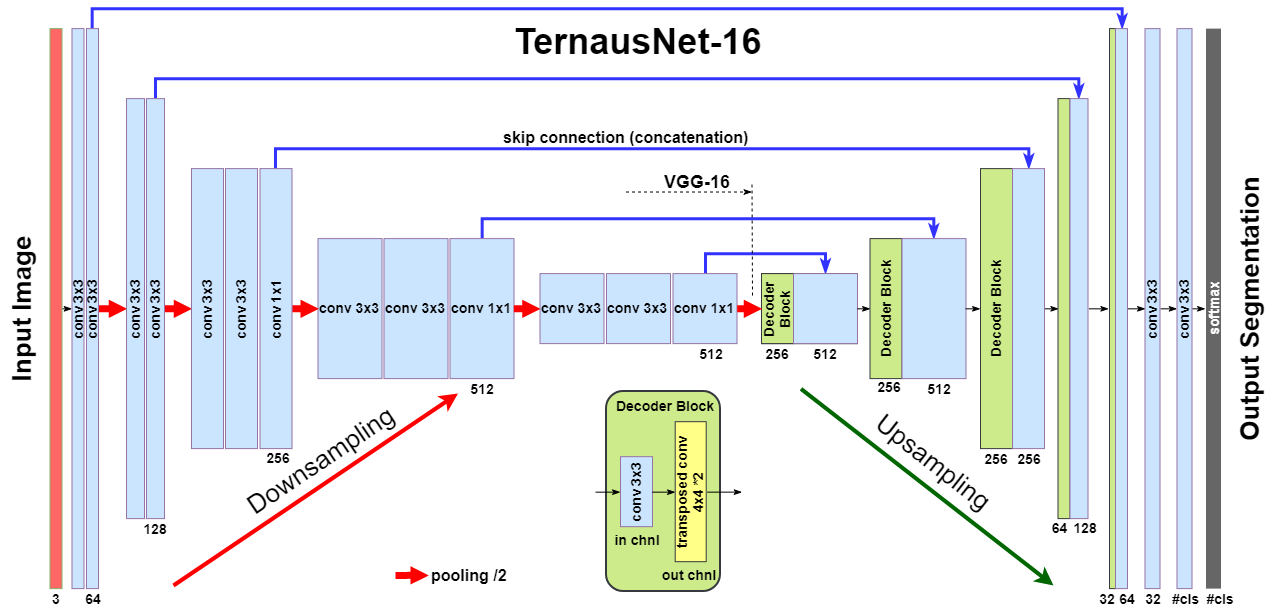
\includegraphics[width=.8\textwidth]{images/networks/TernausNet16.png}
	\caption[TernausNet-16~\cite{Shvets2018}]{Structure of the segmentation network TernausNet-16. 
	Each box corresponds to a multi-channel feature map with the number of channels denoted below the box. 
	The height of each box represents the corresponding feature map resolution. 
	The blue arrows illustrate skip-connections where information is transmitted from the decoder
	to the encoder phase of the network.~\cite{Shvets2018}}
	\label{img:ternausnet16}
\end{figure}

%Localization methods: TRA-KIT, TRA-UGA.
% also: specify localization methods
To solve specifically the localization task of EndoVis15-T, Bodenstedt et al.~\cite{miccai15_results2018bodenstedt} propose two approaches that are not CNN-like: TRA-UGA~\cite{SEG-UGA2016agustinos} and TRA-KIT-RF~\cite{KIT-TRA2016bodenstedt}.

An overview of the previously proposed methods is is given in table~\ref{tab:summary_results_endovis15}

% note: \cite{du2018_2D_pose_est_CNN} doesn't train with challenge guidelines
% Kurmann et al. fehlt!
\begin{table}
\centering
% \small
%\resizebox{!}{1.00cm}{
\begin{tabular}{l c c c c c c c}
\hline\noalign{\smallskip} 
\multicolumn{8}{c}{\textbf{EndoVis15-S results}} \\
 & \multicolumn{2}{r}{b.acc.} accuracy & recall & prec. & spec. & Dice & IoU \\ \hline 
CSL-network~\cite{Laina2017} & 92.6 & - & 86.2 & - & 99.0 &  88.9 & - \\
SEG-KIT-CNN~\cite{KIT-TRA2016bodenstedt} & - &  96 & 77 & 86 & - & 81 & - \\
%network & b.acc. & accuracy & recall/sensitivity & prec. & spec. & Dice & IoU & distance \\
SEG-UGA~\cite{SEG-UGA2016agustinos} & - & 96 & 66 & 95 & - & 78 & - \\
FCN~\cite{garcia2017segm_nonrigid_book} & 83.7 & - & 72.2 & - & 95.2 & - & - \\
FCN-real-time~\cite{garcia2017segm_nonrigid_book} & 88.3 & - & 87.8 & - & 88.7 & - & - \\
ResNet-FCN~\cite{deep_residual_instr_segm2017pakhmov} & 92.3 & - & 85.7 & - & 98.8 & - & - \\
CNN-RNN~\cite{Attia2017_surg_tool_cnn-rnn} & 93.3 & - & 90.4 & - & 96.1 & - & 82.7 \\
\hline 
\end{tabular}
%}
\caption[Results EndoVis15-S, State of the Art]{Results of EndoVis15-S (see section~\ref{sec:endovis15}) for every proposed paper. Balanced accuracy (b.acc.), accuracy, recall, precision~(prec.), specificity (spec.), Dice, Intersection over Union~(IoU) are given in \%. For definition of evaluation metrics see section~\ref{sec:evaluation_metrics}.}
\label{tab:summary_results_endovis15}
\end{table}


% maybe include more from Bodenstedt paper
\begin{table}
\centering
\begin{tabular}{l c c c}
\hline\noalign{\smallskip} 
\multicolumn{4}{c}{\textbf{EndoVis15-T results}} \\
& distance LOSO & distance T4 & distance-total \\ \hline
CSL-network~\cite{Laina2017} & 20.68 & 49.68 & 34.46 \\
TRA-KIT~\cite{KIT-TRA2016bodenstedt} & - & - & 106.6 \\
TRA-UGA~\cite{SEG-UGA2016agustinos} & - & - & 34.9 \\
% TRA-MERGED~\cite{KIT-TRA2016bodenstedt} & - & - & 32.0 \\
%\hline\noalign{\smallskip} 
\shortstack{FCN-det-reg~\cite{du2018_2D_pose_est_CNN} train set\\ \emph{thresh=20px}} & - & - & 3.36 \\
\shortstack{FCN-det-reg~\cite{du2018_2D_pose_est_CNN} test set\\ \emph{thresh=20px}} & - & 6.96 & - \\
\shortstack{FCN-det-reg~\cite{du2018_2D_pose_est_CNN} test set\\ \emph{thresh=30px}} & - & 7.98 & - \\
\end{tabular}
\caption[Results EndoVis15-T, State of the Art]{Results of EndoVis15-T (see section~\ref{sec:endovis15}) for every proposed localization solution. The distance between predicted position of the instrument and labeled ground truth position of the instrument is given in pixels. The evaluations refer to the results for models trained according to LOSO fashion (distance LOSO), the results for models trained with all training sets and tested on the test sets (T4), and to the mean value of the results of both training methods (distance in total).}
\end{table}



%%%% TEST %%%%
%\begin{table}
%\begin{adjustbox}{center=\textwidth}
%\begin{tabular}{l c c c c c}
%\hline\noalign{\smallskip}
% & Dataset1 left/right instr. & Dataset2 & Dataset3 & Dataset4 & mean dist.\\
%\hline\noalign{\smallskip}
%Laina et al. &  $39.0 / 30.8$ & 9.7 & 10.9 & 13.0 & 20.7 \\
%LOC-03 &  $17.58 / 15.15$ & $11.36$ & $10.83 $ & $12.05 $ & $13.85 $\\ [0.5ex] 
%\end{tabular}
%\end{adjustbox}
%\caption{test2}+
%\label{tab:test2}
%\end{table}
%
%\begin{table}
%\begin{tabular}{l c c c}
%\hline\noalign{\smallskip}
% & Dataset5 left/right instr.& Dataset6 left/right instr.& mean dist.\\
% \hline\noalign{\smallskip}
% Laina et al. & 38.4/60.0 & 36.4/63.9 & 49.68\\
%LOC-04 &  $89.80 / 117.91 $ & $ 88.17 / 120.02$ & $106.4 $ \\ [0.5ex]
%\end{tabular}
%\caption{test1}
%\label{tab:test1}
%\end{table}

% \begin{table}
% \centering
% \begin{tabular}{l r}
% \hline\noalign{\smallskip} \\
%  & loc.error  \\ \hline
% Dataset1 &  39.0/30.8\\
% Dataset2 & 9.7\\
% Dataset3 & 10.9\\
% Dataset4 & 13.0 \\
% Dataset5 & 38.4/60.0\\
% Dataset6 & 36.4/63.9\\ \hline
% \hline 
% mean &  24.8/51.6\\ \hline
% \end{tabular}
% \caption{test3}
% \label{tab:test3}
%\end{table}





\chapter{Methods}
\label{cha:methods}

The goal in this work was to develop a CNN architecture that is able to predict surgical instrument segmentation and location in endoscopic images. All networks are evaluated on EndoVis15 (see section~\ref{sec:endovis15}) and EndoVis17-S (see section~\ref{sec:endovis17}) datasets.
When two instruments are visible at the same time in the input video frame, they are not distinguished by the network. This is done in a postprocessing step.

The approach in this work is to use the information learned by a CNN for instrument segmentation to improve the instrument localization task. When transforming the localization ground truth to the same shape as the segmentation ground truth (see section~\ref{sec:heatmaps}), both tasks can share the parameters of the CNN. This seems to be an advantage in comparison to other localization approaches, as showed recently by Laina et al.~\cite{Laina2017}.
  
\section{Instrument Segmentation Network}
\label{sec:TernausNet_11}
In this work, TernausNet-11 is chosen as basis segmentation network and then extended to solve the localization task.
TernausNet-11 (see figure~\ref{img:ternausnet_11}) is proposed in the winning paper of EndoVis17-S by Shvets et al.~\cite{Shvets2018}. 
The encoder part is a VGG11-Network~\cite{simonyan2014vgg} pretrained on ImageNet~\cite{imageNetWinner2012krizhevsky}. Every convolutional layer of the network is followed by a ReLU activation function. 

The output of TernausNet-11 is a binary image, that contains a white segmentation mask where the instrument is located (see figure~\ref{img:model01_dataset2_good_pred}).

\begin{figure}
\centering
\begin{subfigure}[t]{0.49\textwidth}
	\centering
	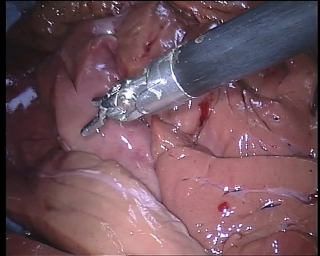
\includegraphics[width=0.65\textwidth]{images/predictions/model01/orig_Dataset2_frame006.jpg}
	\caption{Example input image.}
	\label{img:model01_dataset2_input_image}
\end{subfigure}
\begin{subfigure}[t]{0.49\textwidth}
	\centering
	
\includegraphics[width=0.65\textwidth]{images/predictions/model01/Dataset2_model01_frame006_mask.jpg}
	\caption{Predicted instrument segmentation frame by TernausNet-11.}
	\label{img:model01_dataset2_good_pred}
\end{subfigure}
\caption[Example EndoVis15-S prediction]{Example input image out of EndoVis15-S with corresponding predicted mask by TernausNet-11.}
\label{img:example_segm_pred+gt_unet11}
\end{figure}

As TernausNet-11 outperforms the other networks for the different segmentation challenges except TernausNet-16, which has a larger inference time, TernausNet-11 is chosen as basis for the Localization Network (see section~\ref{sec:tracking_net}).
 
%To solve this task, the segmentation network TernausNet-11~(see section~\ref{sec:TernausNet_11}) is adjusted: It is extended to predict both segmentation and localization of the surgical instruments~(see section~\ref{sec:tracking_net}).

\begin{figure}
	\centering
	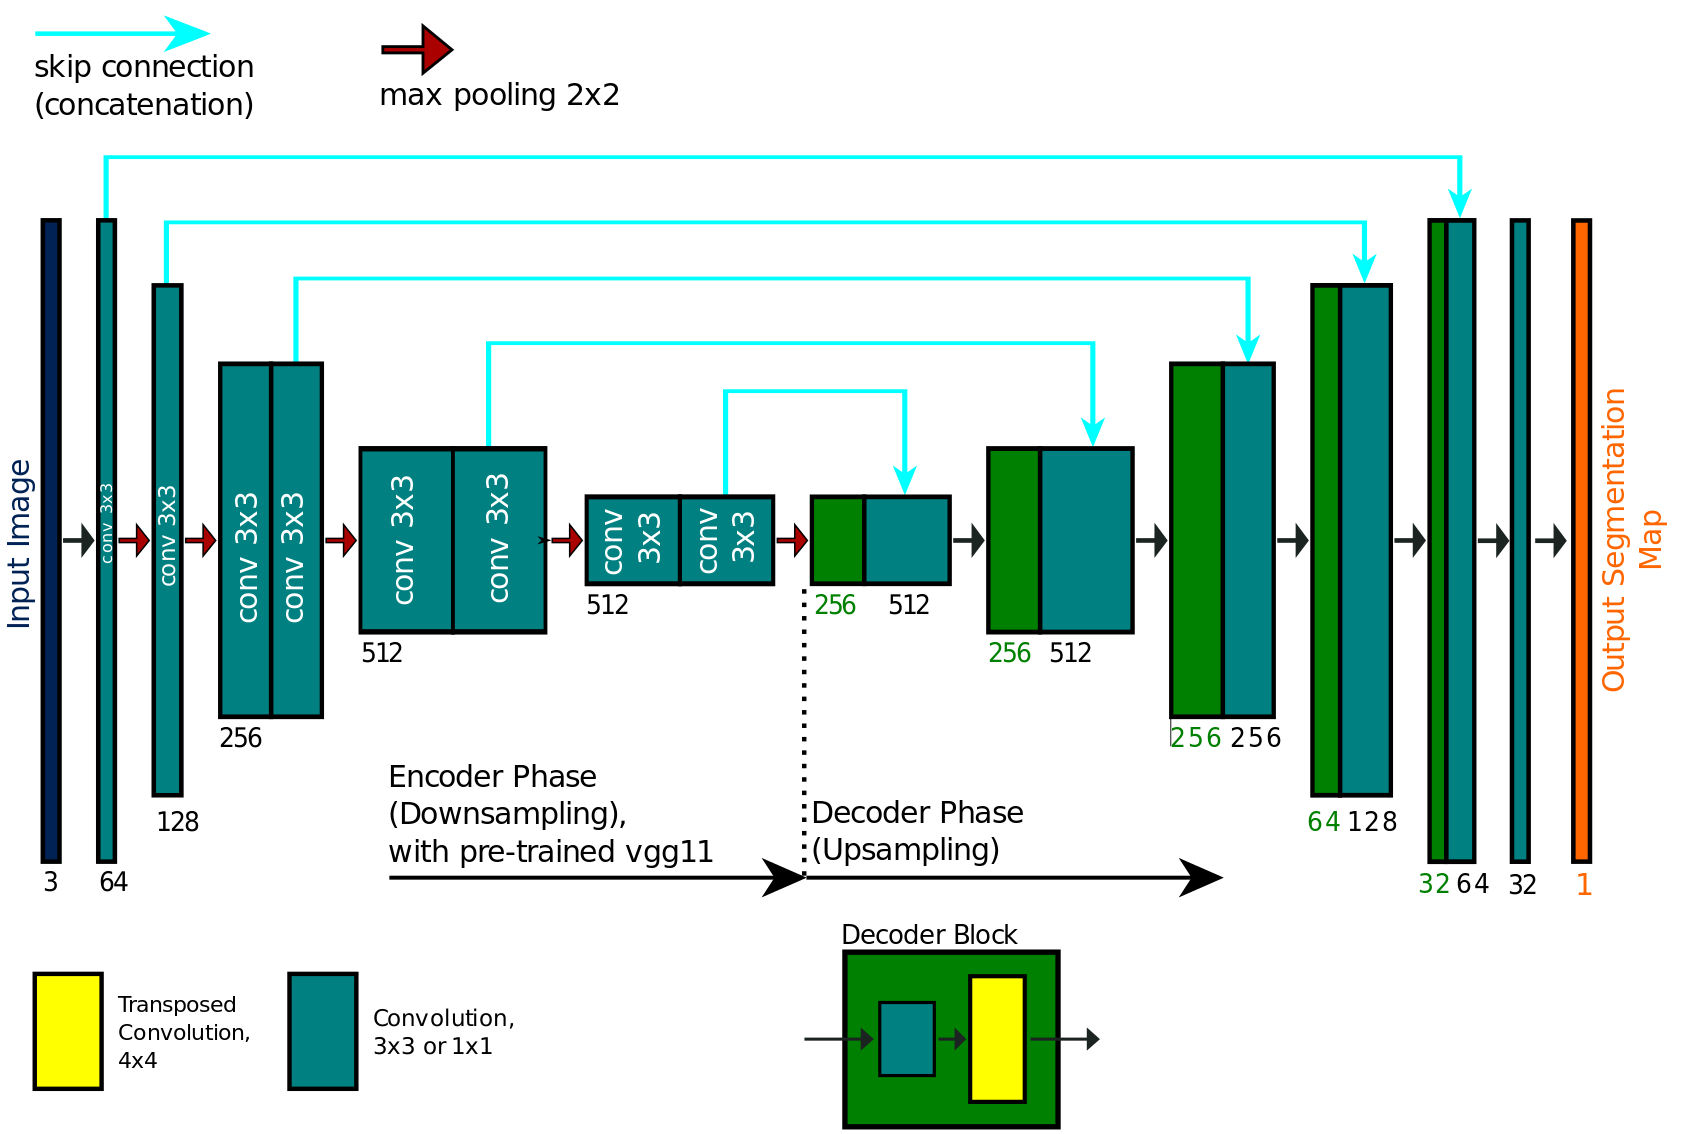
\includegraphics[width=.9\textwidth]{images/networks/TernausNet11_description.png}
	\caption[Structure of TernausNet-11]{Structure of TernausNet-11. The network is proposed by Shvets et al.~\cite{Shvets2018}. 
The blue boxes represent feature maps, the number of channels is denoted below each box. In the decoder phase of the network, each green box is a decoder block that consists of a convolution followed by a transposed convolution. 
The blue arrows denote skip connections:
The feature maps from the encoder phase are concatenated to the decoder blocks in the upsampling phase of the network. 
The red arrows represent 2x2 max pooling operations. The orange box represents the segmentation output of the network.
	}
	\label{img:ternausnet_11}
\end{figure}

TernausNet-11 is trained for the image segmentation task using the loss function $L_{segm}(y_{w,b}(x_j),t_j)$. It consists of two parts:

\begin{equation}
\label{eq:loss_segmentation}
L_{segm}(y_{w,b}(x_j),t_j) = BCE(y_{w,b}(x_j),t_j) - \log J_{binary}(y_{w,b}(x_j),t_j)
\end{equation}

%The first part is the \emph{binary cross entropy (BCE)} loss~(see equation~\ref{eq:bin_crossentropy}), that is combined with a sigmoid function: $BCE_{sigm}$~(see equation~\ref{eq:sigmoid_bin_crossentropy}). 
The first part is a binary cross entropy loss (BCE) combined with a sigmoid function:

\begin{equation}
\label{eq:sigmoid_bin_crossentropy}
BCE_{sigm}(y_{w,b}(x_j),t_j) = -\frac{1}{N}\sum_{i=1}^N{[t_j \log(\sigma(y_{w,b}(x_j)))+(1-t_j)\log(1-\sigma(y_{w,b}(x_j))]}
\end{equation}

Combining the sigmoid function with the BCE loss - instead of applying the sigmoid function first and BCE in a second step - increases the numerical stability.~\cite{murphy2006naive}

The second part of $L_{segm}(y_{w,b}(x_j),t_j)$ is a Jaccard loss for binary evaluation:

\begin{equation} \label{eq:loss_jaccard}
J_{binary}(y_{w,b}(x_j),t_j) = \frac{1}{N} \sum_{i=1}^N \frac{t_j \cdot y_{w,b}(x_j)}{t_j + y_{w,b}(x_j) - t_j \cdot y_{w,b}(x_j)}
\end{equation}

$J_{binary}$ is a differentiable generalization of the Jaccard index that is adjusted to fit into the loss function of the network. It is a differentiable function and therefore suitable for using it for optimizing the network with gradient descent.~\cite{iglovikov2017satellite}

%The Jaccard index~$J(X, Y)$ (see equation~\ref{eq:general_jaccard}) The Jaccard index is taken to measure the similarity of two datasets $X$ and $Y$.

%\begin{equation}
%\label{eq:general_jaccard}
%\begin{aligned}
%J(X, Y) = \frac{\mid X \cap Y \mid }{\mid X \cup Y \mid} &= \frac{\mid X \cap Y \mid}{\mid X \mid + \mid Y \mid - \mid X \cap Y \mid} \\ \\
%0 \le & J(X, Y) \le 1
%\end{aligned}
%\end{equation}

%$J(X, Y)$ is not differentiable and therefore not suitable for using it for optimizing the network with gradient descent. % maybe ref to background  
% 
%
%\begin{equation}
%\label{eq:bin_crossentropy}
%BCE(y_{w,b}(x_j),t_j) = -\frac{1}{N}\sum_{i=1}^N{[t_j \log(y_{w,b}(x_j))+(1-t_j)\log(1-y_{w,b}(x_j))]}
%\end{equation}

\section{Instrument Localization Network}
\label{sec:tracking_net}
The network architecture that is used for localization of surgical instruments in this work is a modified TernausNet-11 (see figure~\ref{img:tracking_network_unet11based}). It is extended by three more layers: One branching layer with 32 channels, one concatenation layer where the segmentation output and the branching layer are concatenated, and one output layer for localization of the instruments.
This architecture is inspired by Laina et al.~\cite{Laina2017}.
The network predicts greyscale images, therefore the segmentation output layer and the localization output layer each have one channel.
The Localization Network is abbreviated as \emph{LocNet}.

The output of the segmentation output layer is the same as the output of TernausNet-11.
The output for the localization task is a greyscale heatmap (see section~\ref{sec:heatmaps}).
A high pixel value at the predicted heatmap indicates a high probability that the instrument center point is located at this pixel position.

\begin{figure}
	\centering
	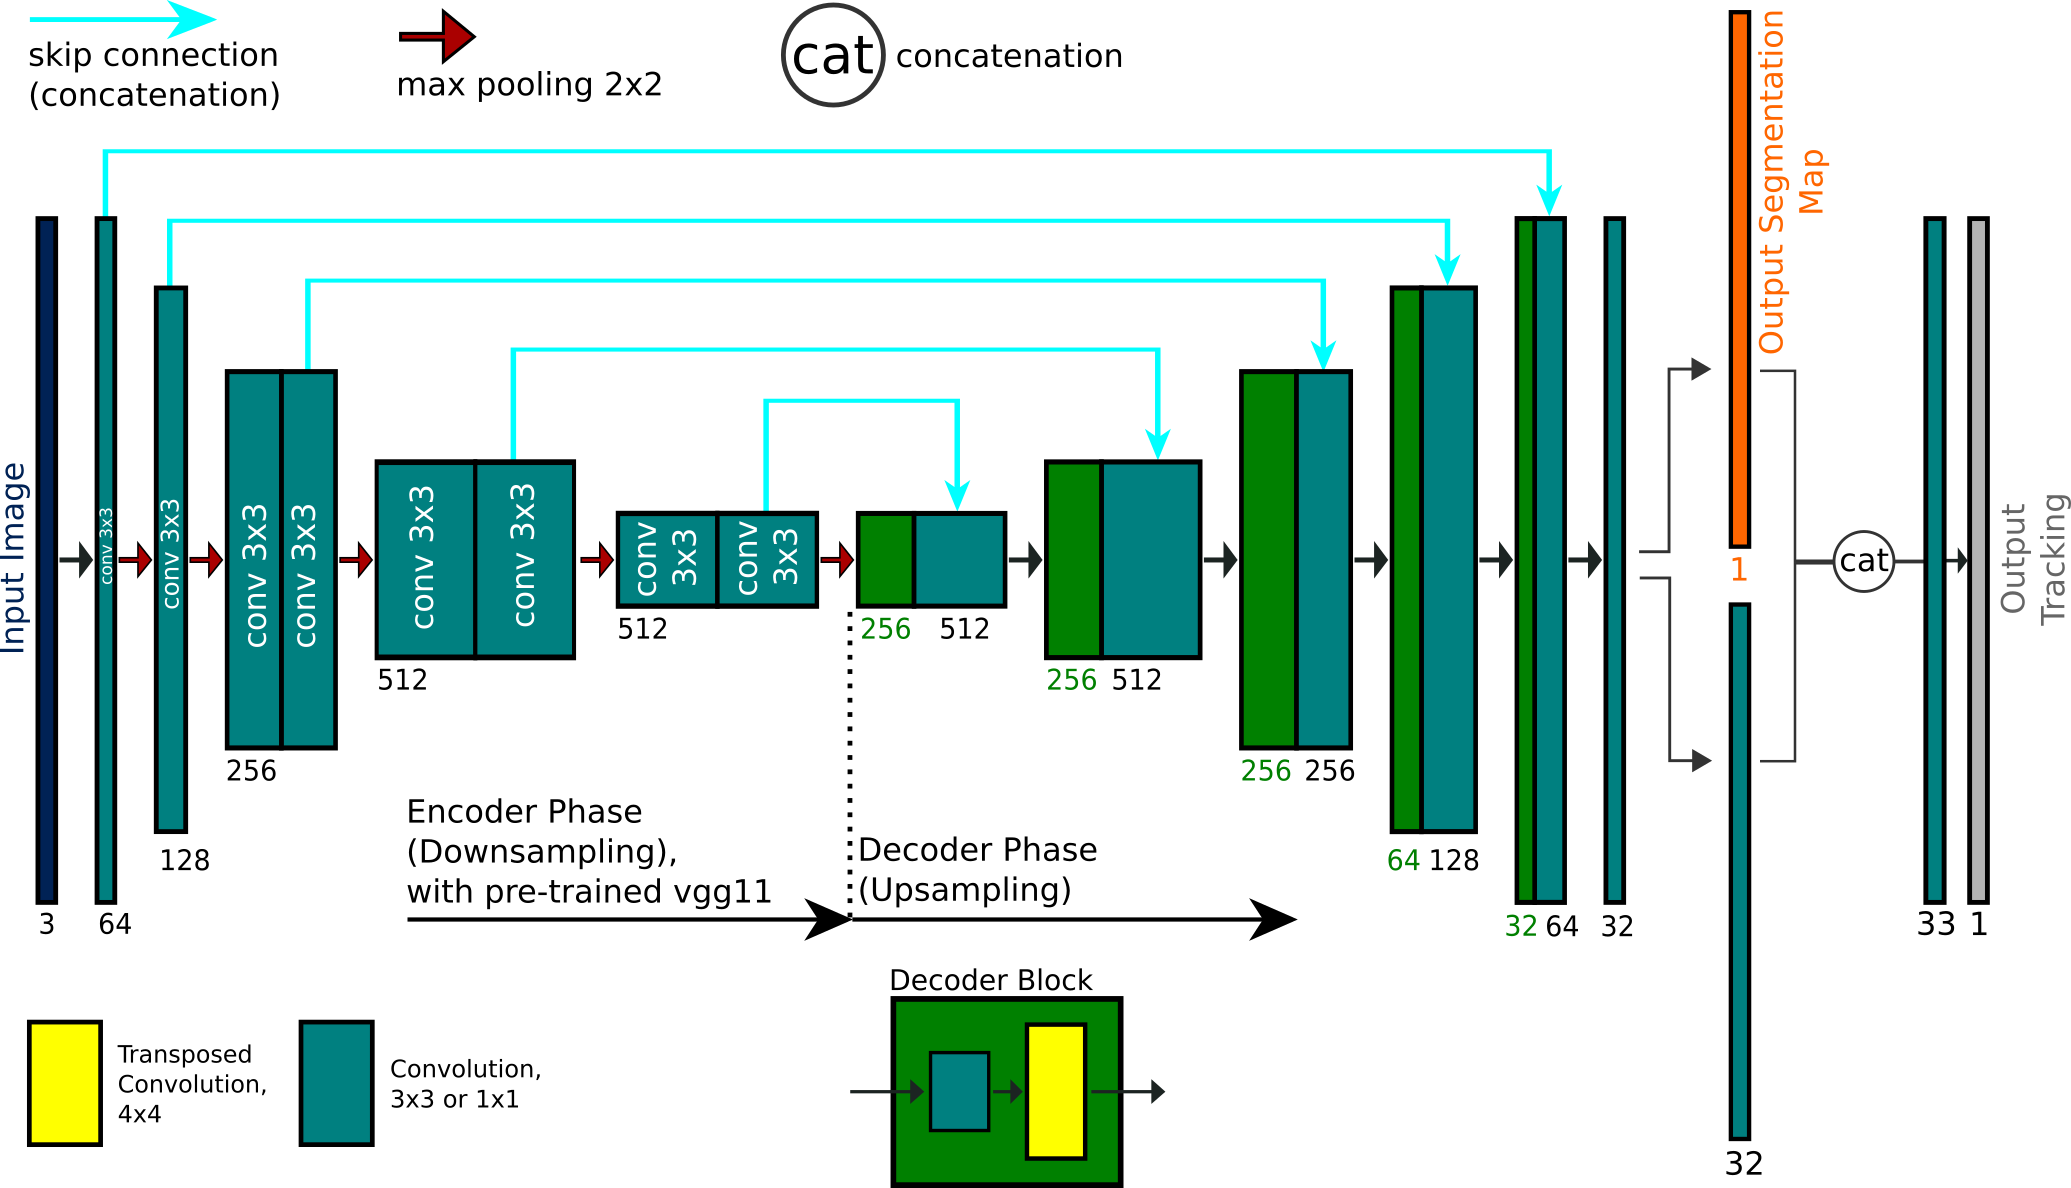
\includegraphics[width=.8\textwidth]{images/networks/TrackingNet_description.png}
	\caption[Structure of Localization Network]{Network architecture that is used for segmentation and localization of the surgical instruments in this work. It is an extended TernausNet-11. The orange box represents the segmentation output, the grey box the localization output of the network.} 
	\label{img:tracking_network_unet11based}
\end{figure}

The output of LocNet is calculated with given input $x_j$ as a tuple $(y_{w,b}(x_j), z_{w,b}(x_j))$, where $y_{w,b}(x_j)$ is the output of the segmentation layer and $z_{w,b}(x_j)$ is the output of the localization layer.
Given the target $s_j$ as ground truth for segmentation and $t_j$ as ground truth for the localization heatmap, a combined loss for concurrent instrument segmentation and localization is defined as follows:

\begin{equation}
\label{eq:track_loss}
L_{loc}(y_{w,b}(x_j), z_{w,b}(x_j), s_j, t_j) := (1-\gamma)L_{segm}(y_{w,b}(x_j), s_j) + \gamma MSE(z_{w,b}(x_j), t_j)
\end{equation}

The segmentation loss is calculated by $L_{segm}(y_{w,b}(x_j), s_j)$, the localization loss is calculated by $MSE(z_{w,b}(x_j), t_j)$. One training sample for segmentation is denoted as $(x_j, s_j)$, one training sample for localization as $(x_j, t_j)$.
The impact of each loss on the overall loss is scaled by the factor $\gamma$.

\section{Heatmaps}
\label{sec:heatmaps}
%gauss function: cite it, explain parameters
It is necessary to convert the localization targets, given 2D image positions for EndoVis15-T, into greyscale images, in order to make it possible for the LocNet to process them.
Out of each localization target one heatmap is created.
The \emph{heatmap} is a greyscale image that has higher pixel values around the center point position of the surgical instrument (see section~\ref{sec:data_preprocessing}).

The heatmaps are generated by calculating a two-dimensional Gaussian distribution $gauss2D(x_r,y_r)$, centered at the center point $(x_{cp}, y_{cp})$ of the instrument.

\begin{equation}
\label{eq:gauss2D_function}
H(x_r,y_r)=gauss2D(x_r,y_r) = \frac{1}{\sqrt{2\pi\sigma^2} } e^{ -\frac{(x_r-x_{cp})^2 + (y_r-y_{cp})^2}{2\sigma^2} }
\end{equation}

The standard deviation $\sigma$ controls the spread of the Gaussian around the instrument location $(x_{cp}, y_{cp})$. $\sigma^2$ denotes the variance. For better interpretability, the pixel values are scaled to the range $[0, 1]$ before given to the network for training.

By iterating over the dimensions of the training input image and applying $gauss2D(x_r,y_r)$, a heatmap with the same dimensions is generated out of the ground truth instrument position.
$(x_r, y_r)$ is one pixel position of the training image, which corresponds to the pixel position in the generated heatmap.


When two instruments are visible in the input image, the heatmap is generated by calculating two Gaussian distributions, one for each instrument (see figure~\ref{img:heatmap_only_2instr}).

\begin{figure}
\centering
\begin{subfigure}[t]{0.49\textwidth}
	\centering
	
\includegraphics[width=.65\textwidth]{images/dataset/robotic15_segm/heatmap_frame001-1instrument.jpg}
	\caption{Example heatmap generated from the ground truth position of one instrument.}
	\label{img:bla}
\end{subfigure}
\begin{subfigure}[t]{0.49\textwidth}
	\centering
	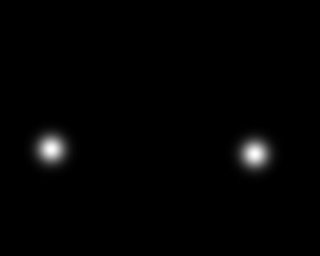
\includegraphics[width=.65\textwidth]{images/dataset/robotic15_segm/heatmap_frame001_2instruments.jpg}
	\caption{Example of a heatmap frame generated for the case of two visible instruments in the corresponding input image.}
	\label{img:heatmap_only_2instr}
\end{subfigure}
\caption[Example heatmap frames]{Example heatmaps generated out of the ground truth for EndoVis15-T.}
\label{img:two_heatmap_frames}
\end{figure}


\section{Postprocessing}
%%%%%% postprocessing%%%%%%
The heatmaps predicted by the network are mostly having a pixel range from $[127,255]$.
In order to improve the extraction of the instrument position, the pixel values of the predicted heatmaps are thresholded with $threshold$ set to 129 (see figure~\ref{img:thresh_pred_loc_model01}): 

\[
    thresh(H(x_r,y_r))= 
\begin{cases}
    H(x_r,y_r)& \text{if } H(x_r,y_r)\geq threshold\\
    0         & \text{otherwise}
\end{cases}
\]

In a second postprocessing step, histogram equalization~\cite{equalization_histogram1987pizer} is used to increase the contrast of the Gaussian distribution in the image (see figure~\ref{img:histogr_pred_loc_model01}).

\begin{figure}
\centering
\begin{subfigure}[t]{0.49\textwidth}
\centering

\includegraphics[width=.65\textwidth]{images/predictions/model1/thresholded-frame001-Dataset2/orig_prediction_frame001.jpg}
\caption{Unmodified localization prediction of LocNet.}
\label{img:pred_loc_model01_unmod}
\end{subfigure}
\begin{subfigure}[t]{0.49\textwidth}
\centering

\includegraphics[width=.65\textwidth]{images/predictions/model1/thresholded-frame001-Dataset2/ONLY_THRESHOLDE_Dataset2.jpg}
\caption{Thresholded localization prediction of LocNet.}
\label{img:thresh_pred_loc_model01}
\end{subfigure}

\begin{subfigure}[t]{0.49\textwidth}
\centering
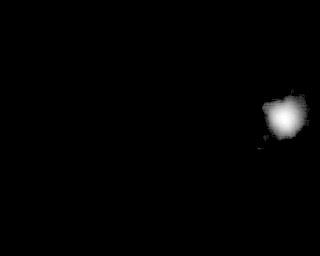
\includegraphics[width=.65\textwidth]{images/predictions/model1/thresholded-frame001-Dataset2/THRESHOLD_and_equalized_Dataset2.jpg}
\caption{Equalized localization prediction of LocNet in order to increase contrast.}
\label{img:histogr_pred_loc_model01}
\end{subfigure}
\begin{subfigure}[t]{0.49\textwidth}
\centering
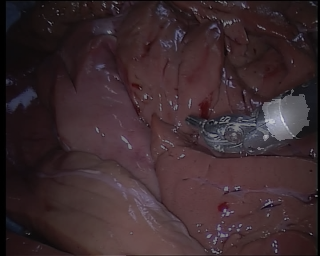
\includegraphics[width=.65\textwidth]{images/predictions/model1/thresholded-frame001-Dataset2/superimposed_preproc_heatmap_frame001.png}
\caption{Input frame out of EndoVis-15 with superimposed postprocessed heatmap.}
\label{img:superimposed_heatmap_thresh_model01}
\end{subfigure}
\caption[Postprocessing steps predicted heatmap]{Example sequence for postprocessing a predicted heatmap. First, the original heatmap (a) is thresholded (b). Afterwards, the contrast is increased by histogram equalization (c). Figure (d) shows the postprocessed heatmap with underlying corresponding input image}
\label{img:threshold_steps}
\end{figure}

%%%%%%% K-MEANS %%%%%%%%%%%%%%
To get the instrument position out of the thresholded heatmap, \emph{k-means} clustering is used. It is a commonly used method to automatically partition a dataset into $k$ groups.~\cite{k-means-paper2005sipkins}
When the input to the corresponding predicted heatmap contains one instrument, $k$ is set to 1. When two instruments are visible in the input image, $k$ is set to 2.
The pixel values of the thresholded heatmap are used as weights for the k-means clustering to improve the results, because a higher pixel value indicates a higher probability that the instrument center is located at that position.

\section{Evaluation Metrics}
\label{sec:evaluation_metrics}
% sources -> already have 2 papers
The following section gives an overview of the evaluation metrics that are commonly used for the validation of NNs. As the network in this work is used for binary classification, the evaluation methods proposed in this section cover only the evaluation of predictions with two classes. The descriptions are adjusted for evaluating LocNet.
There are two classes for binary classification: \emph{Positive} if a pixel in an input image is part of a surgical instrument and \emph{negative} if the pixel belongs to the background. The prediction of a model for one pixel is evaluated as \emph{true} if the predicted class is correct, or \emph{false} if it is wrong. 

Each output predicted by a model can be classified in one of four categories: 

\begin{itemize}
\item $TP\:(true\:positive)$ \\
Represents the number of pixels correctly labeled as surgical instrument.
\item $TN\:(true\:negative)$ \\
Represents the number of pixels correctly labeled as background.
\item $FP\:(false\:positive)$ \\
Represents the number of pixels which are erroneously labeled as surgical instrument but actually are part of the background.
\item $FN\:(false\:negative)$ \\
Represents the number of pixels which are erroneously labeled as background but actually are part of a surgical instrument in the image.
\end{itemize}

The \emph{precision} evaluates the proportion of predicted positive classes ($TP+FP$) that are actually positive classes ($TP$).

\begin{equation}
\label{eq:precision}
\text{precision}=\frac{TP}{TP+FP} 
\end{equation}

The evaluation metric \emph{recall} (see equation~\ref{eq:recall}), in literature also denoted as \emph{sensitivity}, \emph{hit rate} or \emph{true positive rate}, is the proportion of actual positive classes ($TP+FN$) that are correctly predicted as positive ($TP$).~\cite{powers2011eva_recall_precision}
% the amount of all pixels that correspond actually to a surgical instrument - pixels that are correctly identified as instrument ))

\begin{equation}
\label{eq:recall}
\text{recall}=\frac{TP}{TP+FN}
\end{equation}

The evaluation metric \emph{specificity}, also called \emph{true negative rate}, measures the proportion of all pixels that correspond to the negative class ($TN+FP$) that are correctly identified as this class ($TN$).
It can be seen as inverse recall because it works the same way as the recall metric, but takes into account the negative examples instead.~\cite{powers2011eva_recall_precision}

\begin{equation}
\label{eq:specificity}
\text{specificity}=\frac{TN}{TN+FP}
\end{equation}

The evaluation metrics precision and recall focus only on the positive examples and predictions. Neither of them captures information about how the model is handling negative cases.~\cite{powers2011eva_recall_precision}
\emph{Intersection over Union~(IoU)}, also referred to as \emph{Jaccard index}, can be seen as a combination of these two metrics.
It is considered as a better segmentation metric for evaluating binary images because it penalizes both over- and undersegmentation.~\cite{Attia2017_surg_tool_cnn-rnn}
% penalizing oversegm: precision, penalizing under segm: recall

\begin{equation}
\label{eq:iou}
\text{IoU}=\frac{TP}{TP+FP+FN}
\end{equation}

\emph{Dice} (see equation~\ref{eq:dice_binary}) measures the overlap between two binary images~\cite{dice_eva2008babalola}. It is similar to $IoU$, which counts $TP$ only one time in both the numerator and denominator.

\begin{equation}
\label{eq:dice_binary}
\text{dice} = \frac{2 TP}{2 TP + FP + FN}
\end{equation}

\emph{Accuracy} is the proportion of all correct predictions~($TP+TN$) among the total number of cases~($TP+TN+FP+FN$).
The advantage over recall, precision, and $IoU$ is that accuracy explicitly takes into account the classification of negative cases~\cite{powers2011eva_recall_precision}.

\begin{equation}
\label{eq:accuracy}
\text{accuracy}=\frac{TP+TN}{TP+TN+FP+FN}
\end{equation}

The appropriateness of evaluating a model with the accuracy metric depends on the distribution of the dataset. High accuracy results can depend on the distribution of the dataset: Assumed in a surgical instrument dataset the instrument is very small or there are many sequences where no instrument is visible, a model that always predicts the negative case that only background is visible, will achieve high accuracy because the $FN$ rate will be very low.~\cite{metz1987accuracyROC}
% FN rate: erroneously pixels classfied as background but actually belonging to a surgical instrument
% all pixels correctly classified as instrument and background - all pixels in the image
Using \emph{balanced accuracy (b.acc.)} for the evaluation decreases this dependency on the dataset.~\cite{balanced_accuracy2010brodersen}

\begin{equation}
\label{eq:balanced_accuracy}
\text{balanced accuracy}=\frac{1}{2}\left(\frac{TP}{TP+FN}+\frac{TN}{TN+FP}\right)
\end{equation}




\chapter{Evaluation}
\label{cha:evaluation}

\section{Datasets}
In this work, two datasets for segmentation and one for localization of surgical instruments are used for training and testing of the networks. 

\subsection{Endoscopic Vision Challenge 2017}
\label{sec:endovis17}

One segmentation dataset used in this work is part of the subchallenge Robotic Instrument Segmentation of the MICCAI Endoscopic Vision Challenge 2017. The subchallenge is divided into the tasks binary segmentation, part recognition, and type distinction of surgical instruments. 
Binary segmentation means that the instruments are distinguished from the background.~\cite{EndoVis17}
This challenge is abbreviated as \emph{EndoVis17-S}. 

\subsubsection{Robotic Training Data}
\label{sec:endovis17_training}
The eight training sets of EndoVis17-S consist of stereo camera images, each with a resolution of 1280$\times$1024~px (width$\times$height) acquired from a Da Vinci Xi robot~\cite{davindiXI2015morelli} during several different porcine procedures (see figure~\ref{img:original_endovis17_image}).
The ground truth for the camera images are hand annotated 1280$\times$1024~px greyscale images. It is provided for the part and type distinction task. These greyscale images are referred to as \emph{masks}.
For the part recognition task, each instrument part is encoded with different numerical values (see figure~\ref{img:mask_endovis17}).

\begin{figure}
\centering
\begin{subfigure}[t]{0.49\textwidth}
	\centering
	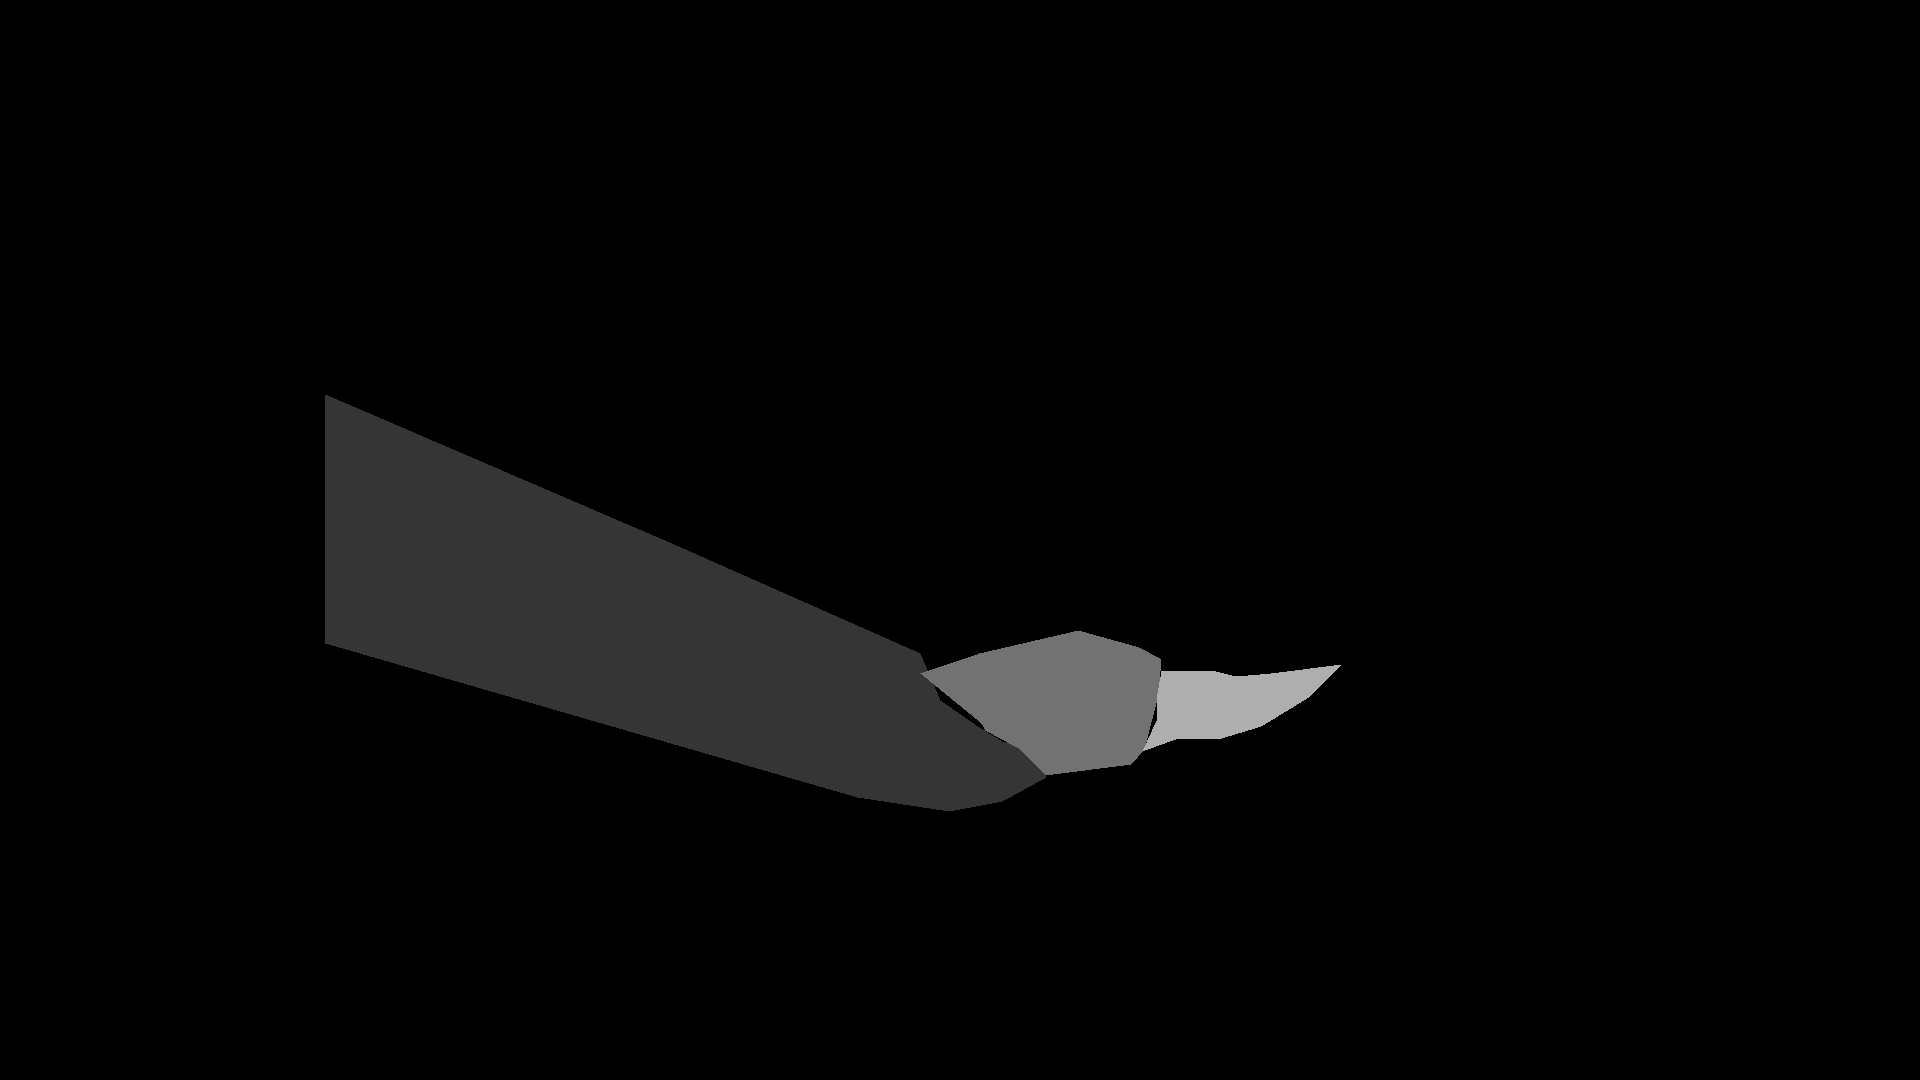
\includegraphics[width=.75\textwidth]{images/dataset/robotic17_segm/high_contrast_map_dataset1_maryland_frame009.png}
	\caption{Example ground truth with increased contrast and brightness for better visibility.}
	\label{img:mask_endovis17}
\end{subfigure}
\begin{subfigure}[t]{0.49\textwidth}
	\centering	
	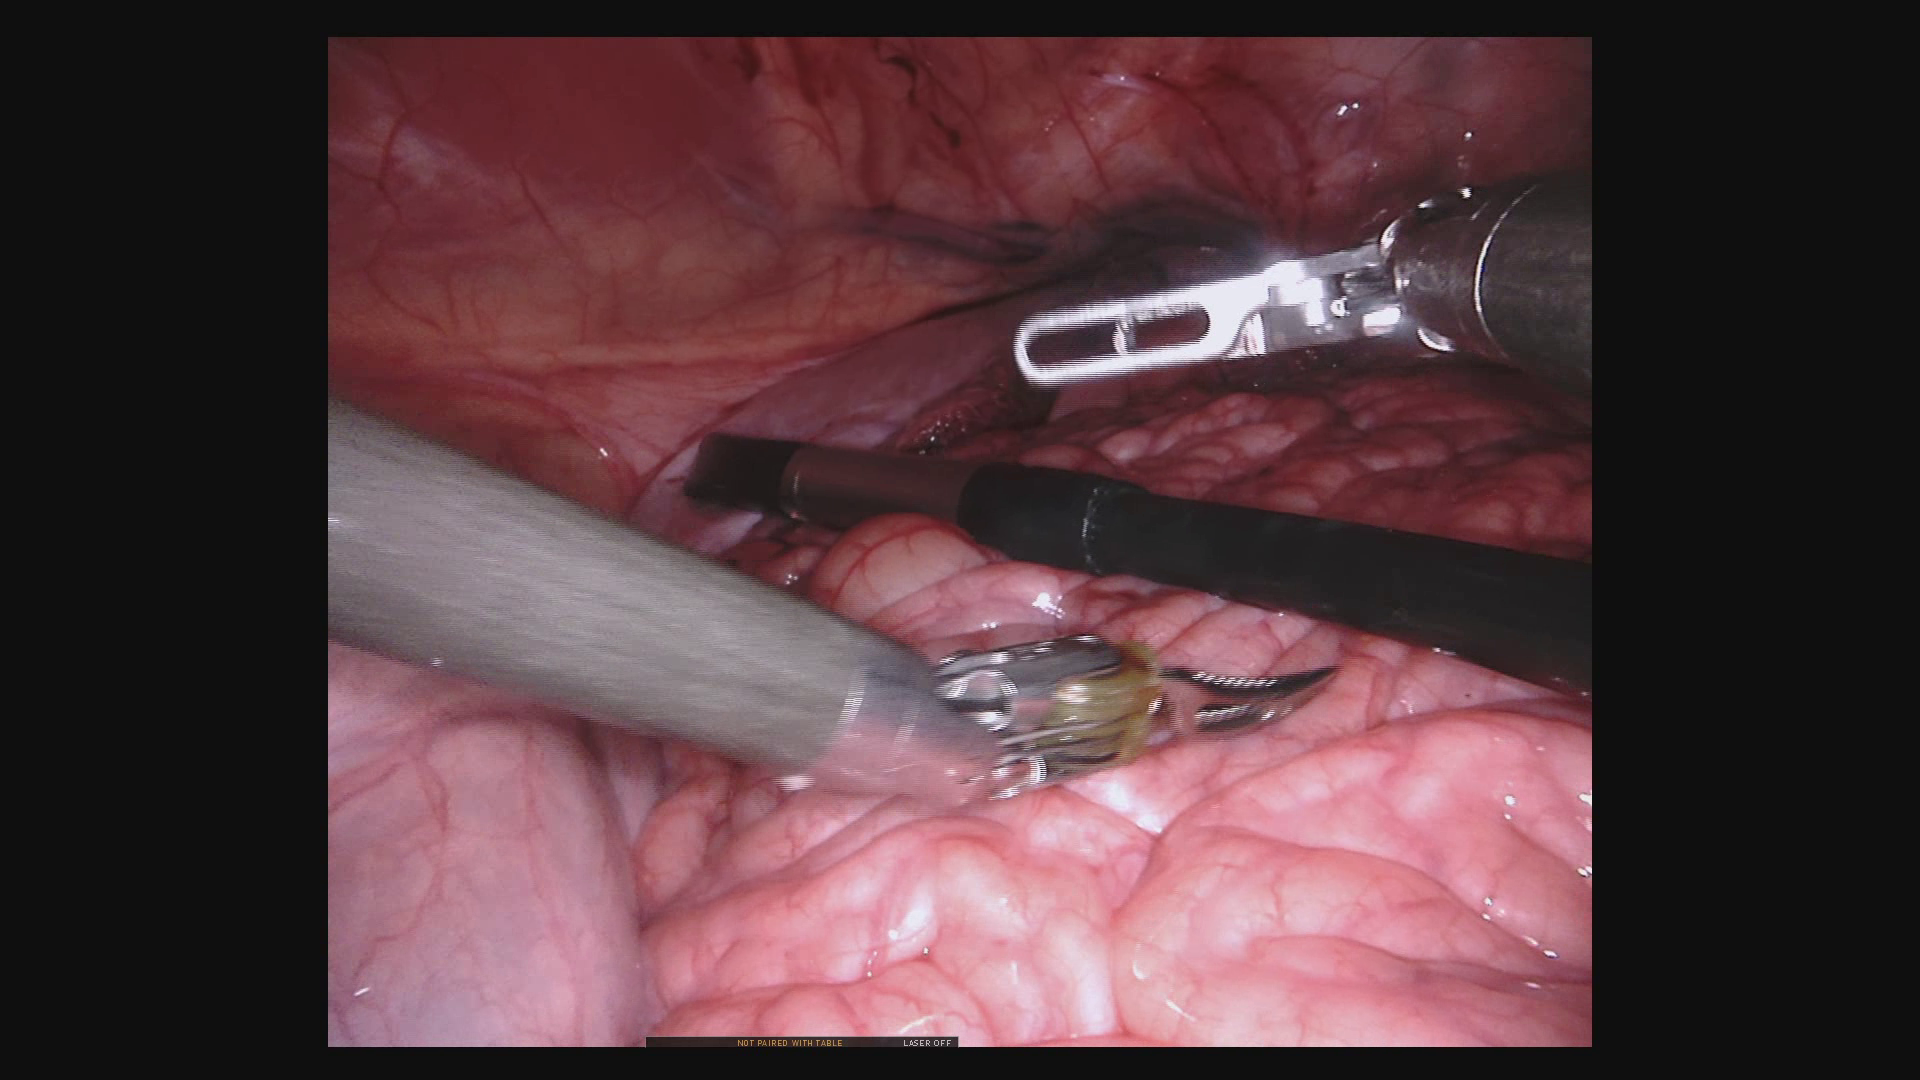
\includegraphics[width=.75\textwidth]{images/dataset/robotic17_segm/dataset1_frame009_3instruments.png}
	\caption{Example image with three instruments visible.}
	\label{img:original_endovis17_image}
\end{subfigure}
\caption[Example data EndoVis17-S]{Unmodified example image and corresponding ground truth for one instrument out of EndoVis17-S.}
\label{img:endovis17_orig_gt_and_image}
\end{figure}

For the instrument type distinction task, the ground truth for each instrument is provided separately: When more than one instrument is visible in the input image, each instrument has one ground truth image (see figure~\ref{img:endovis17_orig_gt_and_image}).

\subsubsection{Robotic Test Data}
The test data consists of eight datasets with 75 images each. They are acquired the same way as the training data. The test sequences were sampled immediately after each training sequence.
Additionally, there are two test sets with 300 images each. They contain different procedures than the eight datasets proposed for training.

\subsection{Endoscopic Vision Challenge 2015}
\label{sec:endovis15}
% decription that these are operation videos
% didn't use rigid -> describe only these ones & explain briefly.
Parts of the data used for this work are proposed in the subchallenge Instrument Segmentation and Tracking of the MICCAI Endoscopic Vision Challenge 2015~\cite{EndoVis15}. The subchallenge in general is abbreviated as \emph{EndoVis15}.

This subchallenge is separated into two dataset types: One \emph{rigid set} that contains only rigid surgical instruments and one \emph{robotic set} that contains only robotic surgical instruments.
The rigid set contains laparoscopic instruments during colorectal surgeries. It reflects typical challenges in endoscopic vision like occlusion, smoke and bleeding. 
In the robotic set, the instruments show typical poses and articulation in robotic surgery.  There is some occlusion, but no smoke and bleeding in any sequence.

This work only uses the robotic set. It is separated in a segmentation and a localization part.~\cite{EndoVis15}
The training and test inputs are the same, the ground truth is different for each part.
The segmentation part is abbreviated as \emph{EndoVis15-S}, the tracking part is abbreviated as \emph{EndoVis15-T}. 

\subsubsection{Robotic Training Data}
\label{sec:endovis15_robotic_train}
There are four robotic training sets. Each consists of a different 720$\times$576~px ex-vivo surgery video with 1100 frames per video and corresponding ground truth for each frame.
\emph{Ex-vivo} refers to procedures that are realized in an artificial environment outside a living organism.
The four surgeries are performed using the Da Vinci Surgical System~\cite{davinci2014watanabe}.

The first training set displays two instruments, the remaining three sets contain one instrument.

For EndoVis-S, the ground truth is provided as a greyscale video. For every frame, the (R,G,B) values of each pixel are labeled as background~(0,0,0), shaft~(160,160,160) or manipulator~(70,70,70) of the surgical instrument.

For EndoVis-T, the ground truth is provided as a text file where clasper angle, center point, and shaft axis of the instrument for every frame is listed (see figure~\ref{example_tracking}).

\begin{figure}
	\centering
	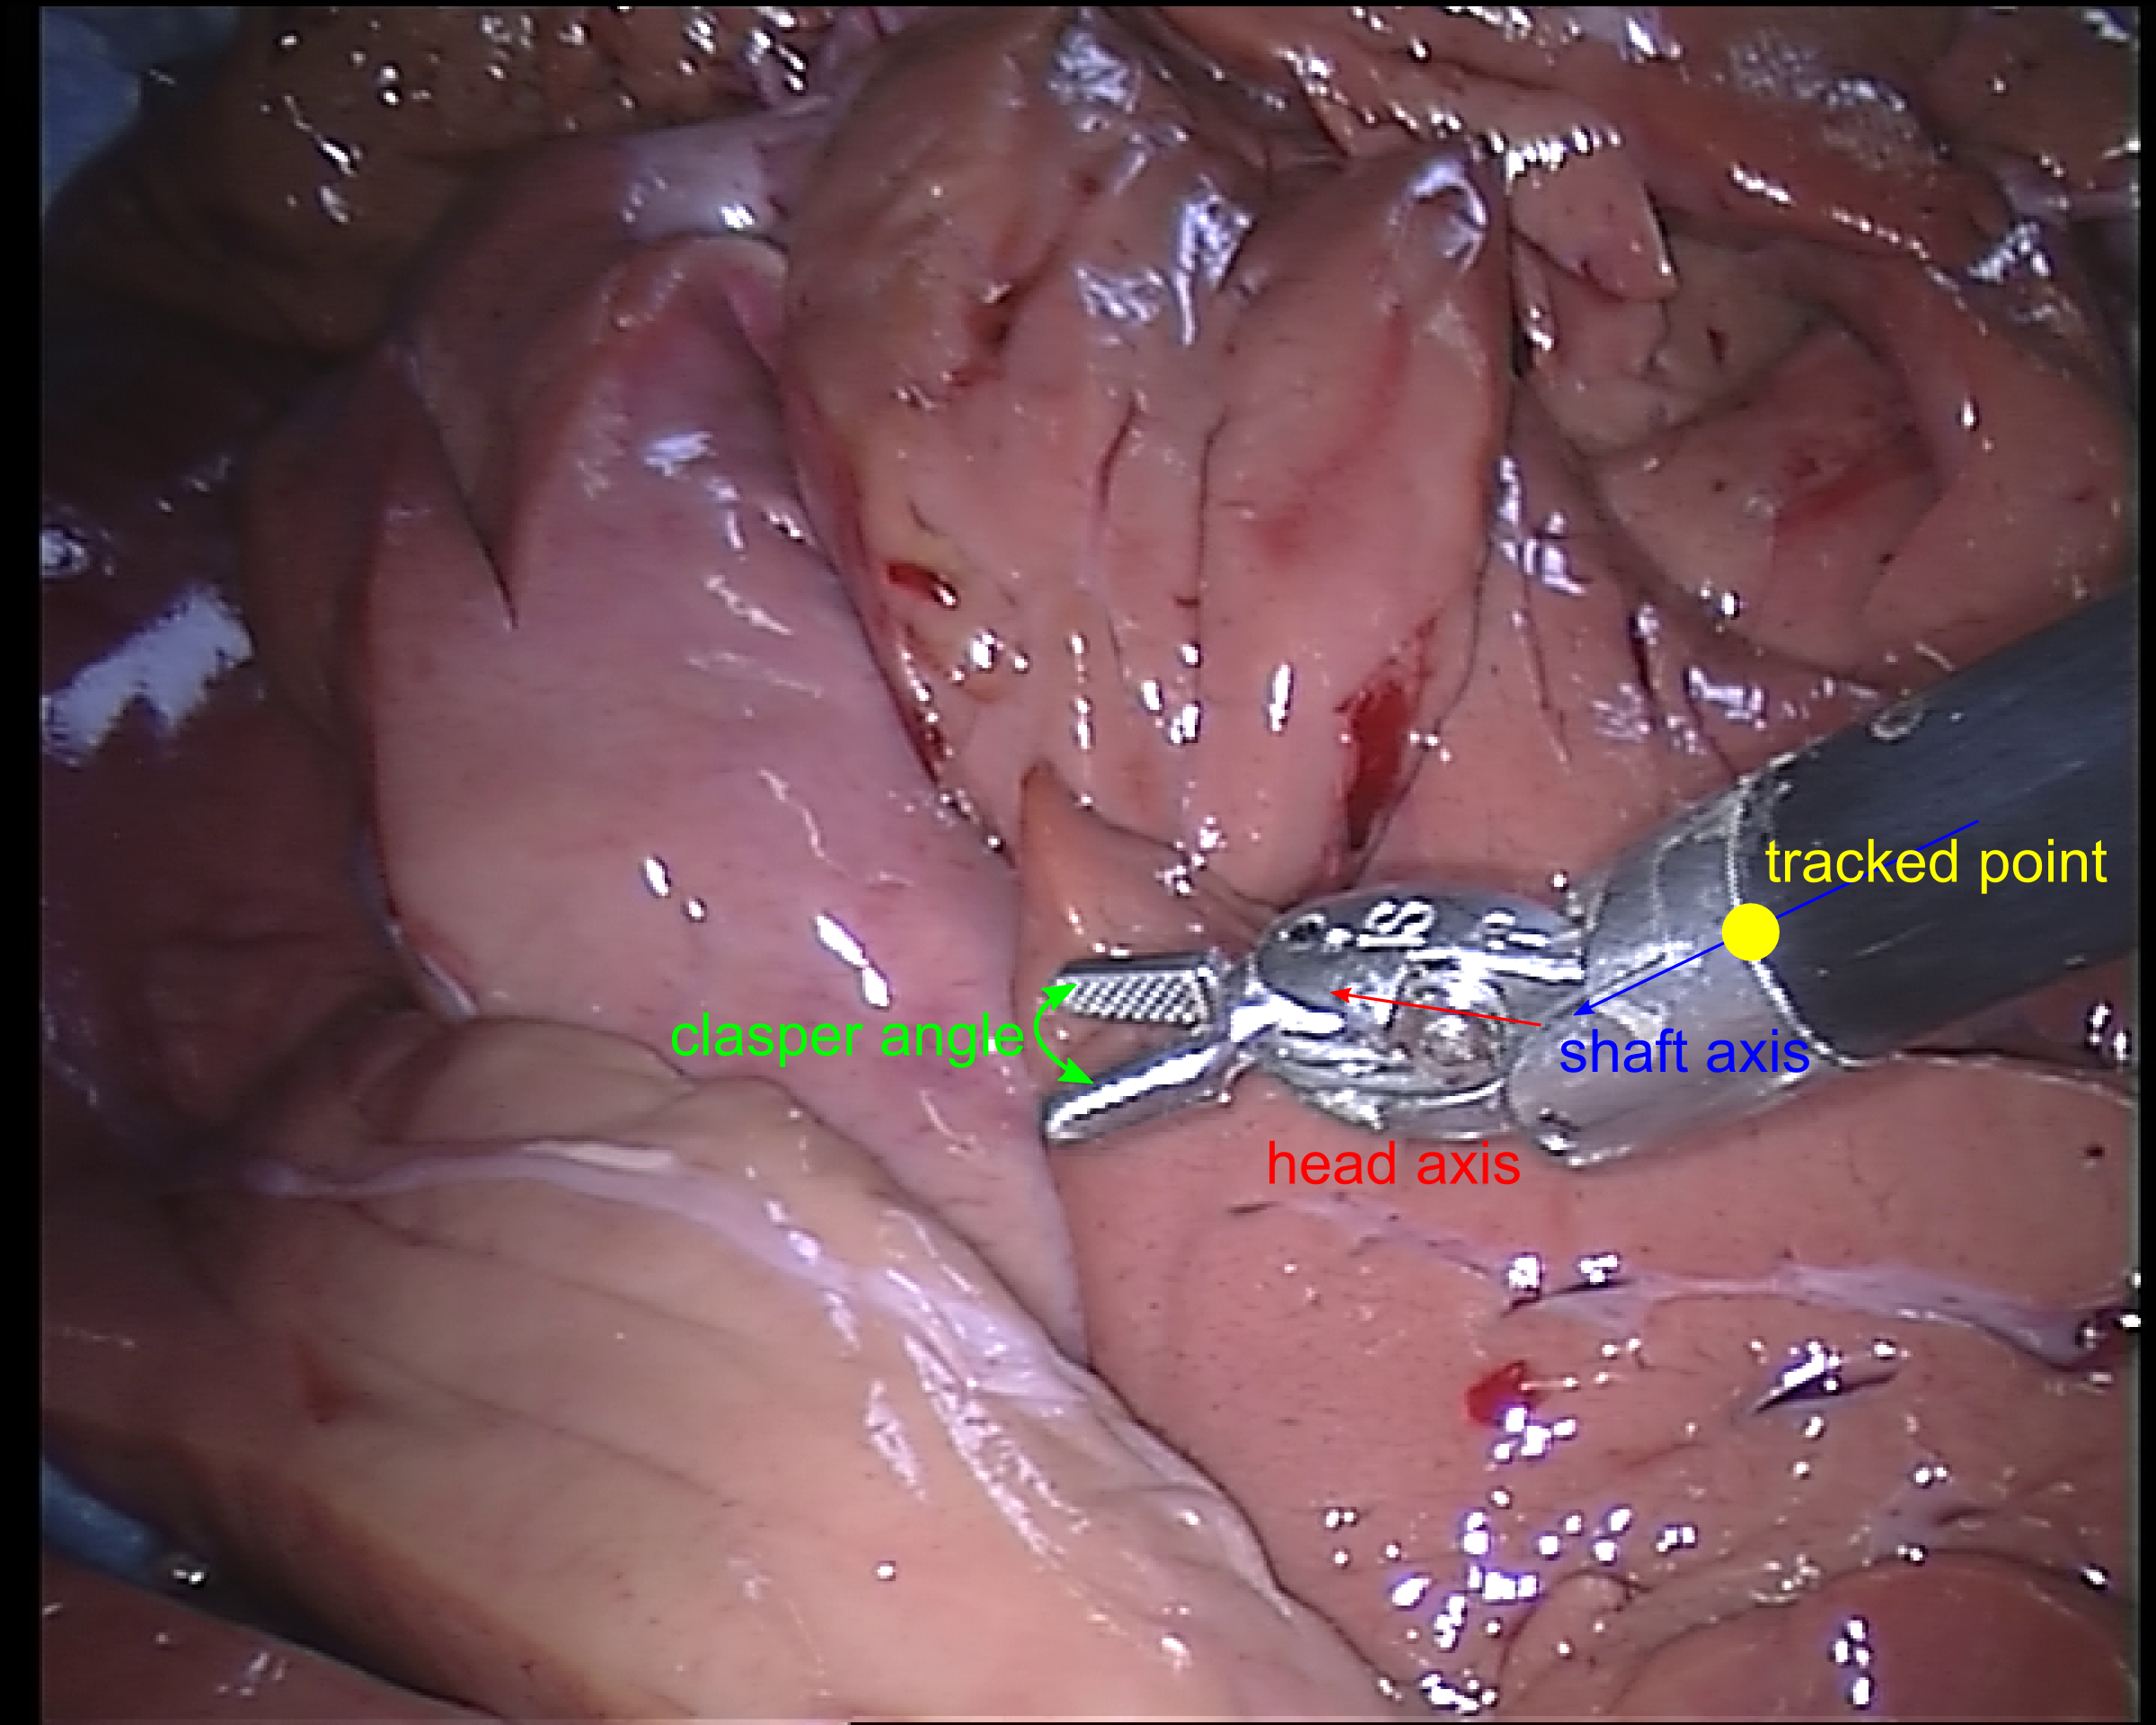
\includegraphics[width=.5\textwidth]{images/dataset/tracking_robotic15/guide_tracking.png}
	\caption[Example ground truth explanation EndoVis15-T]{Example image of EndoVis15-T provided by the challenge administrators to demonstrate the ground truth annotation for localization of the surgical instruments.}
	\label{example_tracking}
\end{figure}

\subsubsection{Robotic Test Data}
\label{sec:endovis15_robotic_test}
The robotic test data consist of 720$\times$576~px frames of additional video material for each of the four surgeries provided for training and two additional recorded surgeries with 1500 frames per video.

The ground truth for testing is provided the same way as for training.

The challenge guidelines specify two methods for testing the trained models.
The first method is a \emph{leave-one-surgery-out fashion (LOSO)}: For each of the four surgeries provided for training, one model is trained with the remaining three surgeries. The performance of the model is tested with the additional testing material for the one surgery that was not used for training. This is similar to $k$-fold cross validation (see also section~\ref{nn:testing}) with $k=4$.

The other testing method consists of training one model with the four surgeries provided for training and testing the performance with the two additional surgeries provided for testing.

\section{Data Preprocessing}
\label{sec:data_preprocessing}
To prepare the datasets for training and testing, several modifications have to be made to fit them for the network. 

\subsection{Endoscopic Vision Challenge 2017}
\label{sec:preprocess_endovis17}
The images of EndoVis17-S are surrounded by a black canvas (see figure~\ref{img:original_endovis17_image}). It is removed by cropping the images. This step is proposed in Shvets et al.~\cite{Shvets2018}
Without canvas, the images have a resolution of 1280$\times$1024~px.
The cropped images are downsampled to a resolution of 320$\times$265~px to decrease training time. 

\begin{figure}
\centering
\begin{subfigure}[t]{0.49\textwidth}
	\centering
	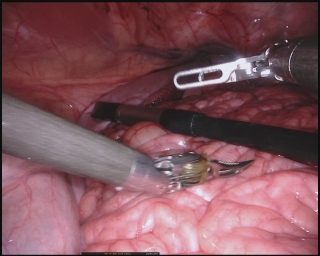
\includegraphics[width=.7\textwidth]{images/dataset/robotic17_segm/frame009_3instr_preprocessed.jpg}
	\caption{Preprocessed example image.}
	\label{img:preprocessed_train_img_segm17}
\end{subfigure}
\begin{subfigure}[t]{0.49\textwidth}
	\centering
	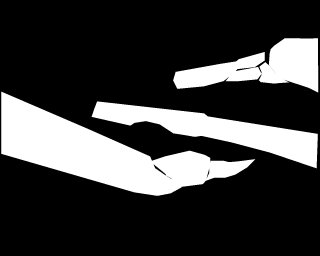
\includegraphics[width=.7\textwidth]{images/dataset/robotic17_segm/merged_dataset1_maryland_frame009.png}
	\caption{Preprocessed example mask: The three different instruments have the same colour.}
	\label{img:preprocessed_mask_segm17}
\end{subfigure}
\caption[Example data EndoVis17-S]{Example data provided for EndoVis17-S.}
\label{img:example}
\end{figure}

\begin{figure}
\centering
\begin{subfigure}[t]{0.49\textwidth}
	\centering
	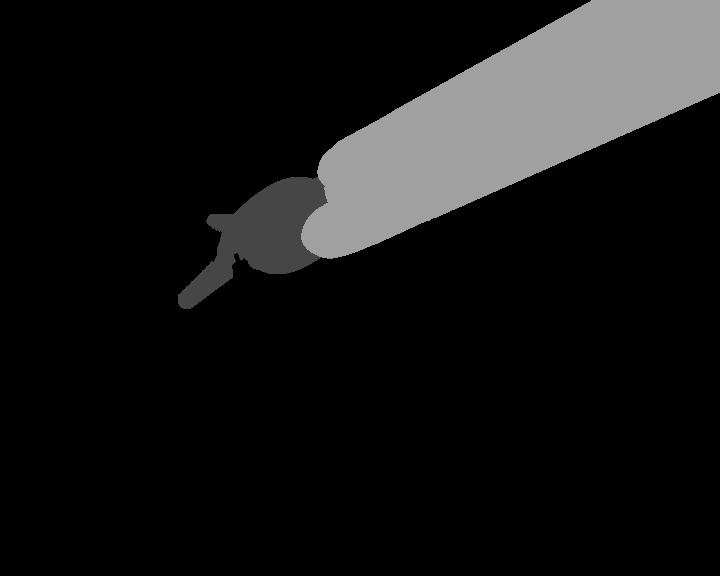
\includegraphics[width=.7\textwidth]{images/dataset/robotic15_segm/mask_original_dataset2_frame0.jpg}
	\caption{Original example mask with part annotations.}
	\label{img:orig_frame_endovis15}
\end{subfigure}
\begin{subfigure}[t]{0.49\textwidth}
	\centering
	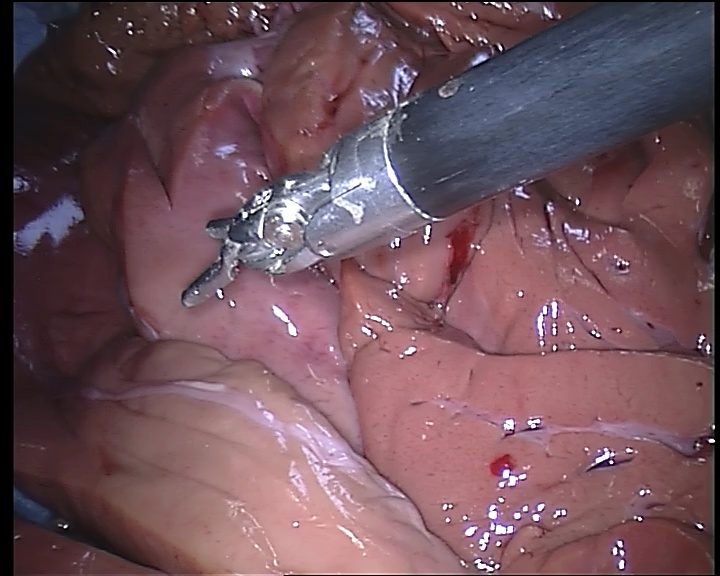
\includegraphics[width=.7\textwidth]{images/dataset/robotic15_segm/img_original_dataset2_frame0.jpg}
	\caption{Original example image.}
	\label{img:orig_mask_endovis15}
\end{subfigure}
\caption[Example data EndoVis15-S]{Unmodified example data provided for EndoVis15-S.}
\label{img:endovis15seg_orig_mask_image}
\end{figure}

Like the corresponding input images, the ground truth masks have a black canvas that has to be removed.
For the part recognition task of EndoVis-S (see figure~\ref{img:mask_endovis17}), the proposed masks have different greyscale values. As the networks in this work solve a binary segmentation problem, the greyscale masks are modified: The different greyscale values are reduced to two values~(R,G,B): Background (0,0,0) and instrument (255,255,255). For the type distinction task, every instrument has one single mask. When there is more than one instrument visible at the same time, their masks are merged into one image. 
After that, one binary mask contains the segmentation ground truth of all instruments shown in the corresponding input image. Like the corresponding input images, the masks are downsampled to a resolution of 320$\times$265~px~(see figure~\ref{img:preprocessed_mask_segm17}).

\subsection{Endoscopic Vision Challenge 2015}
\label{sec:prepocess_endovis15} 
The first preprocessing step for EndoVis15-S is extracting the images and masks out of the proposed videos.    
The resulting input images (see figure~\ref{img:orig_frame_endovis15}) and masks (see figure~\ref{img:orig_mask_endovis15}) have a resolution of 720$\times$576~px.
In order to give the EndoVis15-S data to the same network as the EndoVis17-S data, EndoVis15-S input images and corresponding masks are also downsampled to the resolution of 320$\times$265~px.

To prepare the masks for the binary segmentation task, the same adaptions as for \mbox{EndoVis17-S} are necessary:
The masks with greyscale values are converted into a binary image: Every pixel containing an instrument has the (R,G,B) value (255,255,255). The background pixels have the (R,G,B) value (0,0,0).
When two instruments are shown at the same time in one input image, the corresponding separated masks for each instrument are merged into one mask.

After the conversion to binary masks, erroneous white artefacts surrounding the instrument occur (see figure~\ref{img:white_artefacts_endovis15}).
When applying the operation opening (see Haralick et al.~\cite{opening1987haralick}), the white artefacts are reduced to such a low level that the masks can be used for training (see figure~\ref{img:mask_endovis15_after_morphology}).

\begin{figure}
\centering
\begin{subfigure}[t]{0.49\textwidth}
	\centering
	
\includegraphics[width=.65\textwidth]{images/dataset/robotic15_segm/white_artefacts_dataset1_frame21.jpg}
	\caption{After converting the ground truth images of EndoVis15-S to binary masks, they are surrounded by white artefacts.}
	\label{img:white_artefacts_endovis15}
\end{subfigure}
\begin{subfigure}[t]{0.49\textwidth}
	\centering
	
\includegraphics[width=.65\textwidth]{images/dataset/robotic15_segm/mask_after_morph_dataset1_frame21.jpg}
	\caption{After applying opening operation, the amount of white artefacts surrounding the instruments is reduced.}
	\label{img:mask_endovis15_after_morphology}
\end{subfigure}
\caption[Application opening operation on binary masks]{Binary masks out of EndoVis15-S before and after the application of opening operation~\cite{opening1987haralick}.}
\label{img:unprocessed_processed_masks_endovis15}
\end{figure}

% extracted only FIRST TWO vectors out of Pose.txt
The localization ground truth of the surgical videos is provided as a text file with instrument positions. These instrument positions are each converted into a heatmap, see section~\ref{sec:heatmaps}:
The standard deviation $\sigma$ (see equation~\ref{eq:gauss2D_function}) is set to 25. This way, the resulting Gaussian distribution around the center point of the instrument does not exceed the instrument itself, but is larger than a small point (see figure~\ref{img:superimposed_heatmaps}).

\begin{figure}
\centering
\begin{subfigure}[t]{0.49\textwidth}
	\centering
	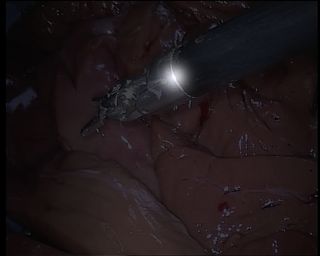
\includegraphics[width=0.7\textwidth]{images/dataset/robotic15_segm/img+heatmap_1instrument.png}
	\caption{Example image with superimposed corresponding heatmap.}
	\label{img:instr+heatmap}
\end{subfigure}	
\begin{subfigure}[t]{0.49\textwidth}
	\centering
	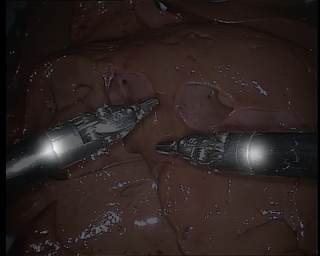
\includegraphics[width=0.7\textwidth]{images/dataset/robotic15_segm/image_frame001_superimposed_heatmap.png}
	\caption{Example image containing two instruments with superimposed corresponding heatmap.}
	\label{img:2instr+heatmap}
\end{subfigure}
\caption[Example image EndoVis15-T, corresponding heatmap]{Example images out of EndoVis15-T with corresponding heatmaps.}
\label{img:superimposed_heatmaps}
\end{figure}

Because the text file with the instrument center points is given for the original images with a size of 720$\times$576~px, the resulting heatmaps have the same size.
To fit them to the downsampled input images, the resolution of the heatmaps is reduced to 320$\times$265 pixels.

\section{Experiments}
After preprocessing the proposed datasets, TernausNet-11 (see section~\ref{sec:TernausNet_11}) and LocNet (see section~\ref{sec:tracking_net}) are trained and evaluated in different ways with EndoVis15-S, EndoVis17-S, and EndoVis15-T.

\subsection{Instrument Segmentation}
% (include example predicted masks)
Because TernausNet-11 is the basis network of LocNet, the segmentation task is evaluated on TernausNet-11 before using the evaluation results to improve the localization task.
The training and testing of the models trained with EndoVis15-S is performed according to the challenge guideline LOSO (see section~\ref{sec:endovis15_robotic_test}) of EndoVis15. All models were trained with batch-size 4.

% model #03: EndoVis15 only
The model \emph{TER-15S} is trained for 100 epochs with learning rate $\lambda=0.0001$ and 100 epochs more with $\lambda=0.00001$ on EndoVis15-S. 

% model #01: EndoVis15 + EndoVis17: 200 epochs 15, +100 epochs 17
% TER = TernausNet
% 15S = EndoVis15 segm set
% 200 = number of epochs
The model \emph{TER-15S-17S} is trained for 100 epochs with $\lambda=0.0001$ and 100 epochs with $\lambda=0.00001$ on EndoVis15-S.
Afterwards it is trained for 100 epochs with $\lambda=0.00001$ on EndoVis17-S. For the training on EndoVis17-S, the eight proposed training sets are divided in four subsets. Each of these subsets contains two training sets. These four subsets are used for training and testing the TER-15S-17S model with LOSO fashion on EndoVis15-S. 

For the results of both TernausNet-11 segmentation models see table~\ref{tab:training_results_seg}.

% Tabelle mit Ergebnissen für TRAININGSDATEN 4-fold (all correct now)
\begin{table}
\centering
 \begin{tabular}{l c c} 
 \hline\noalign{\smallskip}
 \multicolumn{3}{c}{\textbf{Segmentation Results TernausNet-11}} \\
  & TER-15S & TER-15S-17S \\ [0.5ex] 
 \hline
 epochs & 200 & 300 \\ [0.5ex]
% batch-size & 4 & 4 & 4 \\
% method & LOSO & LOSO & LOSO \\ 
 \hline \hline\noalign{\smallskip}
 precision & $92.77 \pm 6.35$ & $92.72 \pm 7.51$ \\
 b.acc. & $89.27 \pm 3.54$ & $88.26 \pm 7.07$ \\
 accuracy & $97.14 \pm 1.35$ & $96.94 \pm 2.04$ \\
 specificity & $99.32 \pm 0.62$ & $99.28 \pm 0.68$ \\
 recall & $79.22 \pm 6.78$ & $77.23 \pm 14$ \\
 IoU & $74.93 \pm 8.41$ & $73.39 \pm 14.29$ \\
 dice & $85.37 \pm 6.15$ & $83.73 \pm 11.32$ \\ [0.5ex]
 \hline
\end{tabular}
\caption[TernausNet-11 segmentation results]{Results of the different models for the segmentation of surgical instruments. Epochs denote the number of epochs for training in total. For evaluation metrics see section~\ref{sec:evaluation_metrics}. The evaluation results are given as mean value over all prediction results $\pm$ the standard deviation.}
\label{tab:training_results_seg}
\end{table}

%%% Discussion
%%% model TER-15S , model TER-15S-17S
The achieved results are comparable to other state-of-the-art approaches. 
TER-15S-17S was trained additionally with data from EndoVis17-S in order to test the impact of additional training data on the prediction performance of LocNet. 
The results for TER-15S and TER-15S-17S for testing on EndoVis15-S are in the same range, i.e. the additional data does not have an impact with high significance on the prediction capability of LocNet for EndoVis15-S. 
As the EndoVis17-S data are obtained during in-vivo procedures with seven different instruments, they differ from the EndoVis15-S data that were obtained in ex-vivo procedures with less different instrument types. Therefore, the information learned by the model out of EndoVis17-S does not have an improving effect on the prediction for EndoVis15-S.

\subsection{Concurrent Instrument Segmentation and Localization}
Each model is trained and evaluated according to one of the EndoVis15-T challenge guidelines: LOSO fashion (see section~\ref{sec:endovis15_robotic_test}), or training on all train sets and then testing on the test sets. 
For the specific training description of each model see table~\ref{tab:training_descr_locnet}.

\begin{table}
\centering
 \begin{tabular}{l c c c } 
 \hline\noalign{\smallskip}
 \multicolumn{4}{c}{\textbf{Training Conditions LocNet}} \\
	& epochs & val.method & $\gamma$  \\ [0.5ex]
 \hline \noalign{\smallskip}
 LOC-01 & 600 & LOSO & $1/2$ \\ 
 LOC-02 & 600 & LOSO & $2/3$ \\ 
 LOC-03 & 50 & LOSO & $1/2$ \\ 
 LOC-04 & 500 & T4 & $1/2$ \\
 LOC-05 & 100 & T4 & $1/2$ \\
 LOC-06 & 400 & LOSO & 1 \\
 LOC-07 & 100 & T4 & 1 \\ 
 LOC-08 & 500 & T4 & 1 \\ [0.5ex]
 \hline 
 \end{tabular}  
\caption[LocNet training conditions]{Validation method (val.method) specifies if the model was trained according to the LOSO fashion (LOSO), or trained completely on the four training sets and tested on the two test sets (T4). The impact of the segmentation and the localization loss on the model is adjusted by $\gamma$ (see section~\ref{sec:tracking_net}).}
\label{tab:training_descr_locnet}
\end{table}

For the segmentation results of all LocNet models see table~\ref{tab:segm_results_locnet}, for the localization results see table~\ref{tab:loc_results_datasets_LOSO} and table~\ref{tab:loc_results_datasets_T4}.

\begin{table}
\centering
 \begin{tabular}{l c c } 
 \hline\noalign{\smallskip}
 \multicolumn{3}{c}{\textbf{Segmentation Results LocNet}} \\
 & {b.acc.} & Dice \\ [0.5ex]
 \hline\noalign{\smallskip}
 LOC-01 & $88.45 \pm 1.8$ &$85.25 \pm 2.4$ \\ 
 LOC-02 & $\mathbf{90.65 \pm 1.7}$ & $\mathbf{87.8 \pm 2.3}$ \\ 
 LOC-03 & $89.75 \pm 4.1$  & $86.83 \pm 6.2$ \\ 
 LOC-04 & $87.45 \pm 2$ & $83.92 \pm 2.8$ \\
 LOC-05 & $89.45 \pm 2$ & $86.32 \pm 2.77$ \\ [0.5ex]
% LOC-06 & - & - \\
% LOC-07 & - & -\\ 
% LOC-08 & - & - \\ [0.5ex]
 \hline 
 \end{tabular}  
\caption[LocNet segmentation results]{Results of the different models for segmentation of surgical instruments. For evaluation metrics see section~\ref{sec:evaluation_metrics}. The evaluation results are given as mean value over all prediction results $\pm$ the standard deviation. As LOC-06, LOC-07, and LOC-08 are trained with loss factor $\gamma=1$, the segmentation results for these models are optimized for localization only.}
\label{tab:segm_results_locnet}
\end{table}

\begin{table}
\begin{adjustbox}{center=\textwidth}
\begin{tabular}{l c c c c c}
\hline\noalign{\smallskip}
\multicolumn{6}{c}{\textbf{Localization Results Datasets LOSO}} \\
 & Dataset1 left/right instr. & Dataset2 & Dataset3 & Dataset4 & mean dist.\\
\hline\noalign{\smallskip}
LOC-01 & $21.24 \pm 12.5 / 17 \pm 10.4$ & $13.45 \pm 5.9$ & $12.73 \pm 5.7$ & $14.22 \pm 23.5$ & $16.27 \pm 19.6$ \\
LOC-02 & $22.65 \pm 31.1 / 15.5 \pm 22.5$ & - & - & - & - \\
LOC-03 &  $\mathbf{17.58 \pm 12.1 / 15.15 \pm 9.4}$ & $\mathbf{11.36 \pm 6.4}$ & $\mathbf{10.83 \pm 6.3}$ & $\mathbf{12.05 \pm 8.9}$ & $\mathbf{13.85 \pm 10.0}$\\ 
LOC-06 &$372.24 \pm 91.7 / 299.62 \pm 251.1$ & $27.66 \pm 109.9$ & $20.47 \pm 82.13$ & $21.48 \pm 80.2$ & $152.5 \pm 207.9$ \\ [0.5ex] 
\end{tabular}
\end{adjustbox}
\caption[LocNet results leave-one-surgery-out]{Results for the different datasets for each LOSO LocNet model. All models were trained according to the LOSO fashion (LOSO).
Mean dist. is the mean distance over all datasets. Dataset1 is distinguished into left and right instrument (left/right instr.).
The evaluation results are given as mean value over all prediction results $\pm$ the standard deviation. The distance between ground truth location and predicted location of the instrument is given in pixels.}
\label{tab:loc_results_datasets_LOSO}
\end{table}


\begin{table}
\begin{tabular}{l c c c}
\hline\noalign{\smallskip}
\multicolumn{4}{c}{\textbf{Localization Results Datasets T4}} \\
 & Dataset5 left/right instr.& Dataset6 left/right instr.& mean dist.\\
 \hline\noalign{\smallskip}
LOC-04 &  $89.80 \pm 101.1 / \mathbf{117.91 \pm 69.0}$ & $\mathbf{88.17 \pm 91.2} / \mathbf{120.02 \pm 68.2}$ & $\mathbf{106.4 \pm 80.4}$\\
LOC-05 & $\mathbf{69.59 \pm 51.6} / 118.15 \pm 73.2$ & $100.15 \pm 118.8 / 120.32 \pm 70.0$ & $111.7 \pm 94.5$\\ 
LOC-07 &  $114.13 \pm 136.8 / 121.51 \pm 78.8$ & $215.36 \pm 225 / 122.23 \pm 73.5$ & $162.04 \pm 163.9$ \\ 
LOC-08 & $121.5 \pm 146.5 / 122.43 \pm 80.9$ & $231.56 \pm 229.3 / 123.5 \pm 77.5$ & $169.7 \pm 169.7$ \\ [0.5ex]
\end{tabular}
\caption[LocNet results tests EndoVis15-T]{Results for the different datasets for each T4 LocNet model. T4 denotes that the models were trained completely on the four training sets and tested on the two test sets.
Each dataset is distinguished into left and right instrument (left/right instr.).
Mean dist. is the mean distance over all datasets. The evaluation results are given as mean value over all prediction results $\pm$ the standard deviation. The distance between ground truth location and predicted location of the instrument is given in pixels.}
\label{tab:loc_results_datasets_T4}
\end{table}

As the instrument positions are extracted from the heatmaps with k-means clustering and k is set to the number of instruments expected to be seen in the input frame, when the number of instruments actually seen in the input frame differs, the localization results are distorted. 
Another problem is that when the center point of an instrument is disappearing for a certain period of frames, but not the complete instrument, the prediction of the model will still contain higher pixel values, yielding a false-positive localization result for the partly visible instrument. This is because the model predicts a Gaussian distribution surrounding the center point, so even when the center point is not visible, the spread of the Gaussian is contained in the prediction (see figure~\ref{img:nearly_disappeared_instr}). 
In this case, comparing the estimated instrument location to the ground truth leads to unreasonably bad results, since the ground truth location for a center point not shown in the image is $(-1, -1)$ and not the actual instrument location. For this reason, the frames where the center point of the instruments is missing according to the ground truth annotation are excluded from evaluation.

To solve the problems in general, further postprocessing steps could be taken:
By checking the distance between the cluster center points, the case when two expected heatmaps are collapsed into one could be recognized, which would indicate that only one of the two instruments is visible.
%could be setting the distance between the predicted center points as a threshold to annotate the center point of one instrument as invisible to solve the k-means clustering problem.
Setting a threshold for the amount of higher pixel values found in the predicted heatmap to recognize frames where the center point is probably missing, could solve the general disappearing instrument problem.

\section{Discussion}
%As the values of the segmentation evaluation are in the range of current state-of-the-art results, 
The models trained according to LOSO fashion vary in number of epochs and the loss factor~$\gamma$.
LOC-01 and LOC-03 only differ in the number of epochs. The evaluation results are in the same range, but LOC-03 trained with 50 epochs outperforms LOC-01 which is trained with 600 epochs. 
The resulting heatmaps for LOC-01 look different from LOC-03 for Dataset1, the spread of the Gaussian distribution contains a higher variance for LOC-01 (see figure~\ref{img:pred_heatmap_high_variance}).

\begin{figure}
\centering
\begin{subfigure}[t]{0.49\textwidth}
\centering

\includegraphics[width=.7\textwidth]{images/predictions/model1/nearly_vanished_instr/frame308_nearly_disappeared.jpg}
\caption{Example heatmap prediction where the instrument center point is not visible in the input image.}
\label{img:nearly_disappeared_instr}
\end{subfigure}
\begin{subfigure}[t]{0.49\textwidth}
\centering

\includegraphics[width=.7\textwidth]{images/predictions/model3/Dataset1-high_variance/frame037_heatmap_high_variance.jpg}
\caption{Example heatmap prediction with high variance.}
\label{img:pred_heatmap_high_variance}
\end{subfigure}
\caption[Example heatmap prediction high variance, example heatmap prediction disappearing center point]{Example of two heatmap predictions: (a) Heatmap prediction where the instrument center point is disappearing. Notably, the prediction does only contain a low range of pixel values because of the missing center point. (b) Heatmap prediction of LOC-01 with high variance.}
\label{img:high+low_variance_heatmaps}
\end{figure}

This indicates that LOC-03 does not find the center point with high certainty, but the resulting location values are still slightly better than for LOC-01. This could be because the distribution of the Gaussians around the center points are still separated sufficiently, so it is possible to determine the center points with k-means clustering with a high accuracy. As LOC-03 is trained with less epochs than LOC-01, this could indicate that LOC-03 generalizes better and LOC-01 is overfitted on the training data.
LOC-02 differs from LOC-01 only in the size of $\gamma$: The impact of the localization loss is $2/3$, the impact of the segmentation loss is $1/3$.
The resulting values for Dataset1 are slightly worse than for LOC-01 and LOC-03. The resulting heatmaps contain Gaussian distributions with high variance.
For LOC-06, $\gamma$ is set to 1, therefore the impact of the segmentation loss is set to 0. It is trained 350 epochs more than LOC-02. For the LOSO method, this model achieves the lowest results, especially for Dataset1. As Dataset1 is the only dataset where two instruments are shown, and therefore LOC-06 tested on this dataset has not seen more than one instrument during training, it is possible that the missing segmentation information makes it more difficult for the network to predict a previously unseen number of instruments.

The models trained according to T4 fashion vary in the number of epochs and the loss factor~$\gamma$.
LOC-04 differs from LOC-05 in the number of epochs, it is trained 400 epochs more than LOC-05. $\gamma$ is set to four for both models, therefore the segmentation and localization loss have the same impact. The results for both models are in the same rage.
The models LOC-07 and LOC-08 are trained with $\gamma=1$, the impact of the segmentation is set to 0. LOC-08 is trained with 400 epochs more than LOC-07. The results for LOC-08 are lower than for the other proposed T4 models.
The evaluation results for the T4 models differ from the results for the LOSO models with an inaccuracy of more than 70~pixels. Notably, the ground truth annotations for the test datasets Dataset5 and Dataset6 seem to be inaccurate: This is stated by the challenge administrators~\cite{Laina2017}, an example can be seen in figure~\ref{img:wrong_test_gt_exampe+pred}. % Dataset5 -> 1st predicted frame LOC-08 / LOC-07, gt annotation for this frame --> merge in gimp

\begin{figure}
\centering
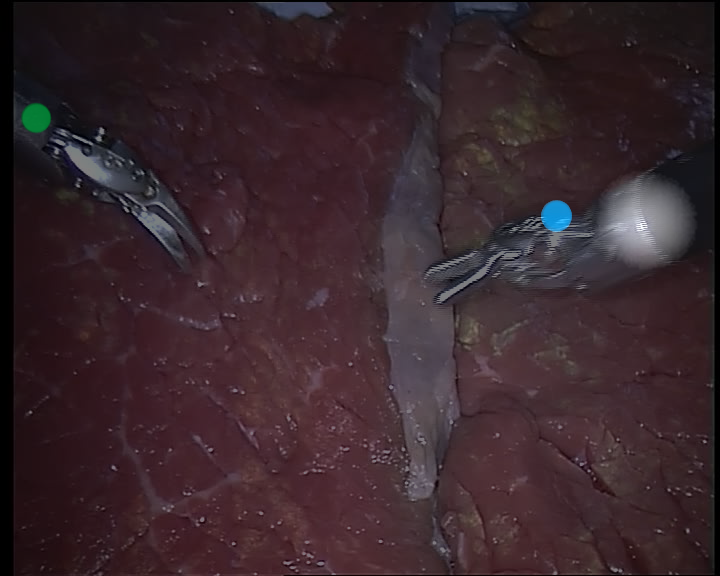
\includegraphics[width=.5\textwidth]{images/predictions/model7/frame001_superimposed_perd_and_gt.png}
\caption[Example image ground truth annotation]{Example input image with superimposed predicted preprocessed heatmap by LOC-07. The given ground truth for the left instrument is denoted in green, for the right instrument in blue. Notably, the center point of the left instrument is not visible, and the center point of the right instrument is actually positioned right from the ground truth annotation.}
\label{img:wrong_test_gt_exampe+pred}
\end{figure}

In summary, the best LOSO model is LOC-03 and the best T4 model is LOC-04. This indicates that setting $\gamma$ to 0.5 yields models with good prediction results.

\subsection{Comparison to State of the Art Methods} 
%The performance of the proposed neural network is compared to other methods using the same dataset and the same evaluation metrics.
The values for segmentation evaluation are in the same range as the current state-of-the-art results, except for the models trained with loss factor $\gamma=1$.

For training method LOSO, the evaluation results for localization outperform the state-of-the-art methods with the models LOC-01 and LOC-03. 
For training method T4, the evaluation results are lower or similar to the state-of-the-art methods.

\subsection{Future Work}
%The localization information obtained by the methods proposed in this work can be used for tracking models. The localization output of the instruments given over time can be used for tracking of surgical instruments during surgery. 
%When the input to the network is occluded by smoke or blood resulting of the surgery procedure, the location of the instrument could still be detected by usind Kalman filtering.
Besides taking further postprocessing steps to improve results, the proposed method could be combined with a temporal tracking algorithm. In this case, the estimated instrument locations could serve as input to trackers such as Kalman filter or Particle filter~\cite{kalman_filter1992brown}. Temporal tracking would be especially helpful to deal with occlusions and to associate each heatmap with either the left or the right instrument, even when instruments cross.

\chapter{Conclusion}
\label{cha:conclusion}

% das habe ich gemacht
In this work, the goal was to obtain a method for segmentation and localization of surgical instruments in endoscopic video frames.
To solve this task, the segmentation CNN TernausNet-11~\cite{Shvets2018} is extended in order to predict localization of surgical instruments in endoscopic videos. This approach was recently proposed by Laina et al.~\cite{Laina2017}.
% Did it meet the required goals defined in introduction chapter? Why/Why not?
% das kam raus / What is the outcome of your evaluation?
All models were trained and evaluated according to LOSO and T4 fashion of the EndoVis15 challenge (see section~\ref{sec:endovis15_robotic_train}),

For the segmentation task, all models trained with loss factor $\gamma < 1$ achieved similar results. The results are in range of the current state-of-the-art methods.
LOC-02 achieved the best segmentation results.

All models trained according to the challenge guideline LOSO achieved better results than the models trained according to the T4 guidelines. The reason is probably that the ground truth annotations for the proposed test datasets are inaccurate, therefore correct predictions of the models are evaluated worse as they actually are.
The model LOC-03 achieved the best prediction results for the LOSO training procedure, it outperforms the current state-of-the-art methods for this evaluation method.
The model LOC-04 achieved the best prediction results for the T4 training procedure. The evaluation results are lower than for current state-of-the-art methods for this evaluation method.

% in Zukunft: für tracking Verfahren nutzen / How can future work improve on your work?
The proposed method could be used in combination with a temporal tracking algorithm in order to serve as input to trackers like Kalman filter or Particle filter.
Temporal tracking would be helpful to deal with occlusions and associate each heatmap in the endoscopic video to the left or right instrument, even when the instrument are crossing.



\cleardoublepage
\listoffigures
\addcontentsline{toc}{chapter}{List of Figures}
\listoftables
\addcontentsline{toc}{chapter}{List of Tables}
%\listofalgorithms
%\addcontentsline{toc}{chapter}{List of Algorithms}
\cleardoublepage

%% --------------------
%% |   Bibliography   |
%% --------------------
\newpage
\addcontentsline{toc}{chapter}{Bibliography}
\bibliography{bibliography}
\bibliographystyle{IEEEtran}
\end{document}
